%%%% Scientific Reports (Nature Portfolio) submission %%%%
%%%% Clean submission copy. Reference style: sn-nature. %%%%
%%%% Add "lineno" to the class options for a line-numbered review copy. %%%%
%%%%
%%%% Every reported number comes from the nested-LOSO run bundle
%%%% five_class_nested_loso_20260807T211827_2b6fb5ac (3 seeds x 5 outer folds).
%%%% Run-dependent figures are regenerated by
%%%%   Code/scripts/evaluate/make_manuscript_figures.py
\documentclass[pdflatex,sn-nature,iicol]{sn-jnl}

\usepackage{graphicx}
\usepackage{multirow}
\usepackage{amsmath,amssymb}
\usepackage{booktabs}
\usepackage{mathrsfs}
\usepackage[title]{appendix}
\usepackage{xcolor}
\usepackage{textcomp}
\usepackage{manyfoot}
\usepackage{indentfirst}

\graphicspath{{./}{figures/}{Figures/}}
\providecommand{\Description}[1]{}

\begin{document}

\title[Audio--EMG Classification of Instructed Jaw Activities]{Audio--EMG Fusion with Dual-Branch Wavelet CNNs for Classifying Instructed Jaw Activities Relevant to Tooth-Contact Bruxism}

\author[1]{\fnm{Mohammad Hassan} \sur{Farhadi}}
\author[1]{\fnm{Ali} \sur{Rabiee}}
\author[1]{\fnm{Rahul} \sur{Singh}}
\author[2,3]{\fnm{Mariusz P.} \sur{Furmanek}}
\author*[1]{\fnm{Reza} \sur{Abiri}}\email{reza\_abiri@uri.edu}
\author*[4]{\fnm{Theodore A.} \sur{Walls}}\email{walls@uri.edu}

\affil[1]{\orgdiv{Department of Electrical, Computer, and Biomedical Engineering}, \orgname{University of Rhode Island}, \orgaddress{\city{Kingston}, \state{RI}, \country{United States}}}
\affil[2]{\orgdiv{Department of Physical Therapy}, \orgname{University of Rhode Island}, \orgaddress{\city{Kingston}, \state{RI}, \country{United States}}}
\affil[3]{\orgdiv{Institute of Sport Sciences, Academy of Physical Education in Katowice}, \orgaddress{\city{Katowice}, \country{Poland}}}
\affil[4]{\orgdiv{Department of Psychology}, \orgname{University of Rhode Island}, \orgaddress{\city{Kingston}, \state{RI}, \country{United States}}}

\abstract{Current consensus defines bruxism as masticatory-muscle activity that may include clenching or grinding with tooth contact and bracing or thrusting without tooth contact. A device that classifies instructed tooth-contact tasks therefore does not, by itself, diagnose bruxism. Here, we report a proof-of-concept engineering study of whether surface electromyography (EMG), audio, and a dual-branch wavelet convolutional neural network can distinguish quiet rest from four instructed jaw-activity classes. Five adults with a prior clinical diagnosis of bruxism completed awake laboratory recordings of rest, jaw movement, clenching, grinding, and chewing. The activities were deliberately performed rather than observed spontaneously. A signal-quality audit showed that the acquisition hardware had already removed the 60-Hz mains fundamental and that 91.3--99.8\% of the in-band power of the previously filtered EMG was residual mains \emph{harmonics}; the analysis was therefore repeated with a harmonic notch bank, trigger-constrained window labeling, and leakage-free nested leave-one-subject-out (LOSO) evaluation. Averaged over the five held-out participants and three training seeds, the fused five-class model achieved 82.1\% accuracy, 73.6\% macro-F1, and a macro one-vs-rest ROC--AUC of 0.962. A sensitivity analysis excluding chewing yielded 79.8\% accuracy and 77.9\% macro-F1 across rest, movement, clenching, and grinding. Collapsing the predictions post hoc into instructed clenching/grinding versus rest/movement/chewing yielded 93.6\% accuracy, an F1 of 87.3\%, and a ROC--AUC of 0.966, with 6.0\% of quiet-rest windows falling into the clenching/grinding group. The modality ablation and the baseline comparison have not been run on the corrected signal and are reported as pending rather than estimated from the superseded pipeline. Including quiet rest allows activity windows to be scored against a non-event condition rather than only against one another. However, the rest data were recorded in a controlled laboratory and do not represent the full range of unrestricted background behavior. No spontaneous awake- or sleep-bruxism episodes were recorded. These results establish only the technical feasibility of multimodal classification of instructed jaw activities and quiet rest in this five-participant dataset; they do not establish continuous free-living event detection, population-level generalization, or clinical validity for diagnosing awake or sleep bruxism.}

\keywords{Jaw-activity classification, Tooth contact, Surface electromyography, Audio sensing, Convolutional neural networks, Wavelet decomposition, Sensor fusion, Powerline interference, Leave-one-subject-out validation}

\maketitle

\section{Introduction}

Bruxism terminology has changed substantially. International consensus no longer defines bruxism simply as involuntary tooth grinding or clenching. Bruxism is a repetitive masticatory-muscle activity characterized by clenching or grinding of the teeth and/or by bracing or thrusting of the mandible~\cite{lobbezoo2018international,verhoeff2025definitions}. Sleep bruxism and awake bruxism are distinct circadian manifestations. Sleep bruxism consists of rhythmic (phasic) or non-rhythmic (tonic) masticatory-muscle activity during sleep, whereas awake bruxism consists of repetitive or sustained tooth contact and/or mandibular bracing or thrusting during wakefulness~\cite{verhoeff2025definitions}. Tooth contact is therefore neither necessary for all bruxism activities nor sufficient to establish that an observed activity is bruxism.

Current frameworks also treat bruxism as a behavior whose clinical relevance depends on the individual and context, rather than as a disorder that is uniformly pathological. Bruxism activities may be neutral, may act as risk indicators for adverse oral-health outcomes, or may have protective associations in some circumstances~\cite{lobbezoo2018international,verhoeff2025definitions}. A recent biopsychosocial model emphasizes that biological, psychological, and social influences interact across the 24-hour cycle and that motor activity cannot be interpreted apart from the person's broader clinical context~\cite{manfredini2026biopsychosocial}. This wider perspective has led to the description of bruxism as a medical gateway for dentistry: careful assessment may connect oral findings with sleep, pain, psychological, medication-related, and other health factors, rather than reducing the problem to dental mechanics alone~\cite{manfredini2024evolution}.

Assessment must therefore be multidimensional. The Standardised Tool for the Assessment of Bruxism (STAB) combines subject-based report, clinical examination, instrumental assessment, possible consequences, and risk or associated factors~\cite{manfredini2024standardised}. Instrumental sensors can contribute objective information about muscle activity, but they represent only one component of this framework. This distinction is particularly important for temporomandibular disorders (TMDs). Bruxism and TMD are not interchangeable diagnoses, and the present study was not designed to evaluate TMD. The INfORM/IADR standard-of-care statement describes TMDs as heterogeneous, multifactorial biopsychosocial conditions whose diagnosis requires validated history and clinical assessment and whose management should generally be patient-centered, conservative, and reversible~\cite{inform2025tmd}. Accordingly, the presence of a jaw-muscle pattern alone should not be presented as a diagnosis of TMD or as proof that bruxism caused a patient's pain or dysfunction.

Recent surveys and educational reports show why precise terminology matters. Dental practitioners use heterogeneous bruxism assessment and management strategies, and outdated beliefs remain common even among trainees~\cite{mungia2025approaches,nasanen2026competence}. Similar educational gaps have been documented for TMDs~\cite{sangalli2026education}. Engineering studies can help address an important measurement problem, but only if the output of a classifier is separated clearly from a clinical diagnosis.

Instrumental assessment outside the clinic remains technically challenging. Surface EMG is sensitive to masticatory-muscle activation but can respond similarly to functional and non-functional activities. Audio may add information about tooth contact and mastication, but it is also sensitive to ambient noise and raises privacy considerations. Natural behaviors fluctuate within and across days; ecological momentary assessment (EMA) studies have therefore used repeated sampling in the natural environment rather than relying on a single retrospective report~\cite{bracci2018frequency,colonna2025fluctuation}. Proposed research routes for awake-bruxism metrics combine subject-based, clinically based, EMA, and instrumental approaches and emphasize matching the measurement method to the research question~\cite{bracci2024metrics}. Multi-day, 24-hour EMG recording has also been proposed for characterizing muscle activity in the home environment~\cite{colonna2023electromyographic}.

Against this background, the present study addresses a narrow engineering question. It does not evaluate spontaneous awake bruxism, sleep bruxism, disease severity, TMD, or treatment response. Instead, it tests whether an audio--EMG system can distinguish quiet rest and four instructed jaw activities performed in a controlled laboratory by five adults with a prior clinical diagnosis of bruxism. The activity labels describe the experimental conditions, not independently adjudicated bruxism episodes.

A second, methodological point motivates this study. Instrumental studies of masticatory-muscle activity are reported almost exclusively through summary accuracies, and the measurement chain that produced them is rarely auditable. During the preparation of this analysis, a spectral audit of our own recordings showed that the conventional preprocessing recipe applied to them---notch the mains fundamental, then band-pass---had removed the one frequency the acquisition hardware had already suppressed and had left the mains \emph{harmonics}, which carried the overwhelming majority of the in-band power, entirely intact. We report that finding, its correction, and its effect on the results, because a classifier trained through such a channel can appear to work while separating interference rather than physiology.

The study addresses three research questions:

\begin{itemize}
    \item \textbf{RQ1:} Can off-the-shelf surface EMG and microphone sensors provide signals that support five-class classification of quiet rest, jaw movement, clenching, grinding, and chewing?
    \item \textbf{RQ2:} Within this dataset, how much does audio add to EMG, and is the improvement concentrated in the chewing class?
    \item \textbf{RQ3:} Does a dual-branch CNN with modality-specific wavelet decomposition outperform the evaluated single-pathway and conventional baselines under the same leave-one-subject-out protocol, including when the task is collapsed to instructed clenching/grinding versus the three comparison conditions?
\end{itemize}

RQ1 is answered below. RQ2 and RQ3 are \emph{not} answered here. Both were previously estimated from runs that used the defective filter chain; those estimates are withdrawn rather than restated, and the confirmatory modality ablation and baseline sweep on the corrected signal are prespecified but have not been run. Where an interim indication exists, it comes from a declared screening harness and is labeled as such throughout.

\section{Prior technical advances}

\subsection{EMG-based assessment}

Surface EMG is widely used for ambulatory assessment because it measures masticatory-muscle activation directly~\cite{raez2006techniques}. Early portable systems established the feasibility of home recording but had limited specificity for distinguishing target activity from other orofacial activity~\cite{stuginski2016detection}. Castroflorio et al.~\cite{castroflorio2013use} combined EMG and electrocardiographic information to identify sleep-bruxism episodes in a natural environment.

Machine-learning studies have reported high performance on controlled tasks, although direct comparison is difficult when labels, participants, and validation protocols differ. Sonmezocak and Kurt~\cite{sonmezocak2021detection}, for example, reported greater than 90\% accuracy using EMG features across jaw opening, clenching, rhythmic grinding, and fatigue/pain classes. Gul et al.~\cite{gul2024advanced} evaluated sleep-related recordings across postures, while Heyat et al.~\cite{heyat2020computational} combined several physiological modalities. Lan et al.~\cite{lan2022comparative} described different surface-EMG patterns during centric and eccentric instructed activities. These studies support technical feasibility but do not make their reported accuracies interchangeable, because some classify pre-segmented tasks whereas others aim to identify events within continuous recordings.

\subsection{Acoustic and wearable sensing}

Acoustic sensing may complement EMG when oral activities produce different sound patterns. Romano et al.~\cite{romano2024wearable} showed that signals from voluntary oral behaviors depend strongly on transducer location and identified ear-adjacent placement as promising for longer recordings. Martinot et al.~\cite{martinot2021artificial} used mandibular-movement analysis to identify phasic sleep-bruxism events in patients with obstructive sleep apnea. Patented systems have also used adaptive sound thresholds or chin-mounted accelerometers~\cite{haugland2020automatic,patwa2017bruxism}. For sleep applications, however, portable devices require comparison with an appropriate sleep reference method; a controlled awake-task classifier cannot be assumed to transfer to sleep~\cite{cidverdejo2024instrumental}.

\subsection{Signal processing and deep learning}

Wavelet decomposition is well suited to non-stationary EMG because it preserves joint time--frequency information~\cite{englehart2003robust}. Wavelet features have performed well in EMG classification~\cite{phinyomark2012feature}, and filter design remains important for preserving physiological content while suppressing noise~\cite{chowdhury2013surface}. CNNs can learn local patterns in physiological signals~\cite{faust2018deep,tsinganos2019improved}. Focal loss and class-weighting methods can reduce the influence of class imbalance~\cite{lin2017focal,johnson2019survey}. The remaining engineering gap addressed here is whether modality-specific wavelet branches improve classification of quiet rest and the four instructed activities in the present dataset.

Surface-EMG reviews consistently identify powerline interference as the dominant environmental artifact and recommend notch filtering combined with a band-pass stage~\cite{chowdhury2013surface,raez2006techniques}. That recommendation is usually implemented as a single notch at the supply frequency. It is only valid when the supply fundamental is in fact the dominant interference. Head-mounted electrodes with long leads, in a laboratory containing displays, lighting and switched-mode supplies, can instead pick up a harmonic-rich waveform, and some acquisition systems apply their own fixed notch before the data reach the analysis software. In that combination the textbook chain removes nothing and still looks correct on a filter-response plot. Verifying the filter against the measured spectrum of the actual recordings---rather than against its own design---is therefore a necessary step, and it is the step added here.

\section{Methods}

This proof-of-concept study was approved by the Institutional Review Board of the University of Rhode Island (Protocol \#IRB22275690-2). All methods were performed in accordance with relevant institutional guidelines and regulations. Written informed consent was obtained from every participant, including consent to publish the identifying image in Fig.~\ref{fig:sensor_setup}.

\subsection{Participants and study scope}

Five adults (2 women and 3 men; age $38.0 \pm 10.4$ years) were recruited through flyers, messages to local oral-care and physical-therapy providers, and word of mouth. Eligibility required a prior clinical diagnosis of bruxism. The study did not independently re-diagnose or phenotype that history, and the available study records did not stratify participants by sleep bruxism, awake bruxism, grinding, bracing, or thrusting predominance. The prior diagnosis therefore describes the sample but is not a reference standard for the activity labels used in this analysis.

All analyzed tasks were performed intentionally while participants were awake in the laboratory. The study did not record spontaneous awake-bruxism episodes or sleep. Consequently, the labels ``clenching'' and ``grinding'' below refer to instructed task performance. They should not be interpreted as natural or independently verified bruxism episodes.

\subsection{Experimental procedure}

The session began with written consent and a pre-screening survey. Surface EMG electrodes, an omnidirectional microphone, and a camera were positioned and secured. Participants first completed 1 minute of quiet rest. They then performed five repetitions of jaw opening/closing, left/right deviation, protrusion/retrusion, and left/right biting. This was followed by 1-minute trials of isometric molar and incisor clenching, alternating 3 seconds of activity with 3 seconds of relaxation.

After a break, participants completed 3-minute trials of instructed grinding, chewing cheese, chewing baby carrots or popcorn, and chewing gum. Each task was repeated three times, with a 1-minute rest between repetitions. A handheld button transmitted event markers synchronized with the physiological recordings. Participants pressed the button at task initiation, and the experimenter visually confirmed task onset.

\subsection{Window labeling and analyzable sample}

The button and task protocol established experimental task labels, not clinical bruxism labels. Every analyzed window is required to lie \emph{wholly inside} one interval during which the trigger marks the participant as actively performing the named task, so that no window can span two conditions or a trigger transition. Windows are cut from the continuously filtered recording, never filtered individually, because filtering each window separately injects an edge transient exceeding one signal standard deviation into the first 50 samples of every example.

Three exclusions are applied before windowing. A \textbf{transition guard} of 0.25~s is removed on each side of every trigger edge. The choice was measured rather than assumed: over 432 task onsets (358 with a detectable envelope transition) the median lag between the button press and the electromyographic onset was $-0.075$~s, muscle activity preceded the marker at 79.9\% of onsets, and among the 20\% of onsets in the harmful direction the median lag was 0.054~s and the largest ever measured was 0.352~s. A \textbf{startup guard} of 0.5~s is removed at the beginning of every recording, replacing an earlier unexplained 3-s skip; amplifier settling transients were observed in 66 of 100 recordings, all settled within 0.40~s, with peak excursions up to $12{,}580\times$ the recording's robust scale. Finally, quiet-rest windows are drawn only from the five dedicated rest recordings; trigger-off intervals inside active recordings are \emph{not} treated as rest, because they are unlabeled rather than verified as quiet.

The resulting rest class represents quiet laboratory rest only. It does not sample the full range of everyday non-event behaviors and therefore does not turn this window classifier into a validated continuous detector.

\subsection{Sensors and dataset}

Four differential surface-EMG channels were recorded from two bilateral bipolar electrode pairs, one pair per side of the head. The tentative electrode map records them as left masseter, left temporalis, right masseter, and right temporalis. One omnidirectional microphone was positioned near the temporomandibular joint (Fig.~\ref{fig:sensor_setup}). All signals were sampled at 1200~Hz. The acquisition chain documented no physical calibration for either modality, so all amplitudes in this paper are reported in arbitrary analog-to-digital converter units and are deliberately not labeled \textmu V, Pa, or dB.

\begin{figure}[h]
  \centering
  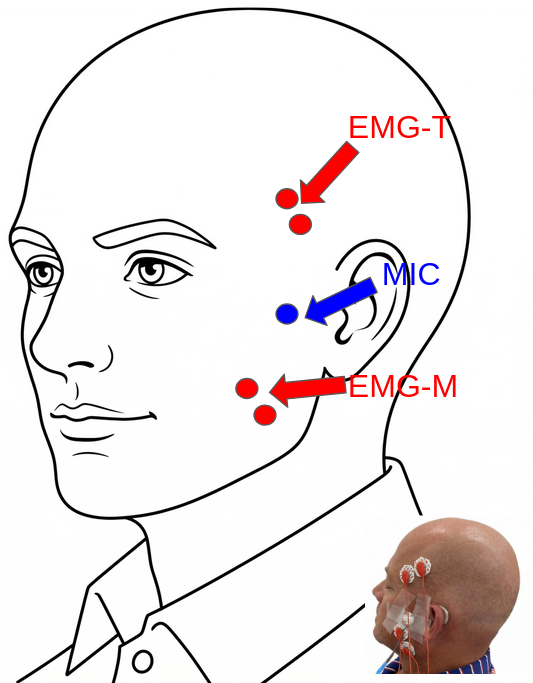
\includegraphics[width=0.9\linewidth]{Figures/patient_new.png}
  \caption{Sensor placement for multimodal data acquisition. Bipolar surface-EMG electrode pairs were positioned over the temporalis (EMG-T) and masseter (EMG-M) muscles. A microphone (MIC) was secured near the temporomandibular joint. This arrangement was evaluated only during instructed awake laboratory tasks.}
  \Description{A participant with surface-EMG electrodes over the jaw muscles and a microphone positioned near the temporomandibular joint.}
  \label{fig:sensor_setup}
\end{figure}

The recordings were consolidated into five experimental classes. \textbf{Rest} comprised windows from the five dedicated quiet-baseline recordings only; as described above, inter-trial intervals inside active recordings were not admitted. \textbf{Movement} included opening/closing, lateral deviation, and protrusion/retrusion. \textbf{Clenching} included molar clench, incisor clench, and unilateral left/right bite. \textbf{Grinding} included the instructed grinding trials. \textbf{Chewing} included cheese, carrots or popcorn, and gum. These categories were selected to contrast quiet non-event periods, static loading, lateral tooth-contact activity, non-chewing jaw movement, and functional mastication. They were not intended as a comprehensive taxonomy of bruxism. In particular, mandibular bracing and thrusting without tooth contact were not elicited as distinct classes.

Chewing was included because it is a common functional activity and a plausible confound for an ambulatory jaw-activity classifier. Because it may also be comparatively easy to recognize, the primary five-class results are accompanied by a sensitivity analysis that excludes chewing. A second analysis collapses the five labels into instructed clenching/grinding versus rest/movement/chewing.

Continuous signals were segmented into 1.0-second windows (1200 samples) with a 0.5-second stride (600 samples), creating 50\% overlap between adjacent windows. Under the containment and guard rules above, 100 recordings yielded 6,173 analyzable windows from 99 recordings: 590 rest, 333 movement, 799 clenching, 816 instructed grinding, and 3,635 chewing (Table~\ref{tab:dataset}, Fig.~\ref{fig:sample_flow}). These counts supersede the 11,845 windows reported previously, which were produced by a legacy policy that labeled whole recordings rather than trigger-verified intervals and therefore included inter-trial and transition material inside activity classes. The two sets of counts are not comparable, and only the trigger-constrained counts are used here.

These windows are not independent observations: adjacent windows overlap by 50\%, many windows originate from the same recording, and all of them originate from only five participants. The participant, rather than the window, therefore defines the effective unit for generalization, and all primary metrics below are computed within a participant before being summarized.

\begin{table}[h]
  \caption{Dataset characteristics under the trigger-constrained labeling policy.}
  \label{tab:dataset}
  \centering
  \small
  \begin{tabular*}{\columnwidth}{@{\extracolsep{\fill}}ll@{}}
    \toprule
    Property & Value \\
    \midrule
    Participants & 5 \\
    Recordings (contributing) & 100 (99) \\
    EMG channels & 4 (2 bilateral pairs) \\
    Microphone channels & 1 \\
    Sampling rate & 1200 Hz \\
    Signal units & Arbitrary ADC units \\
    Window size & 1200 samples (1.0 s) \\
    Stride & 600 samples (0.5 s) \\
    Transition guard & 0.25 s each side \\
    Startup guard & 0.5 s per recording \\
    Rest windows & 590 \\
    Movement windows & 333 \\
    Clenching windows & 799 \\
    Grinding windows & 816 \\
    Chewing windows & 3,635 \\
    Total analyzed windows & 6,173 \\
    Experimental classes & 5 \\
    Quiet-rest class & Included \\
    \bottomrule
  \end{tabular*}
\end{table}

\begin{figure*}[h]
  \centering
  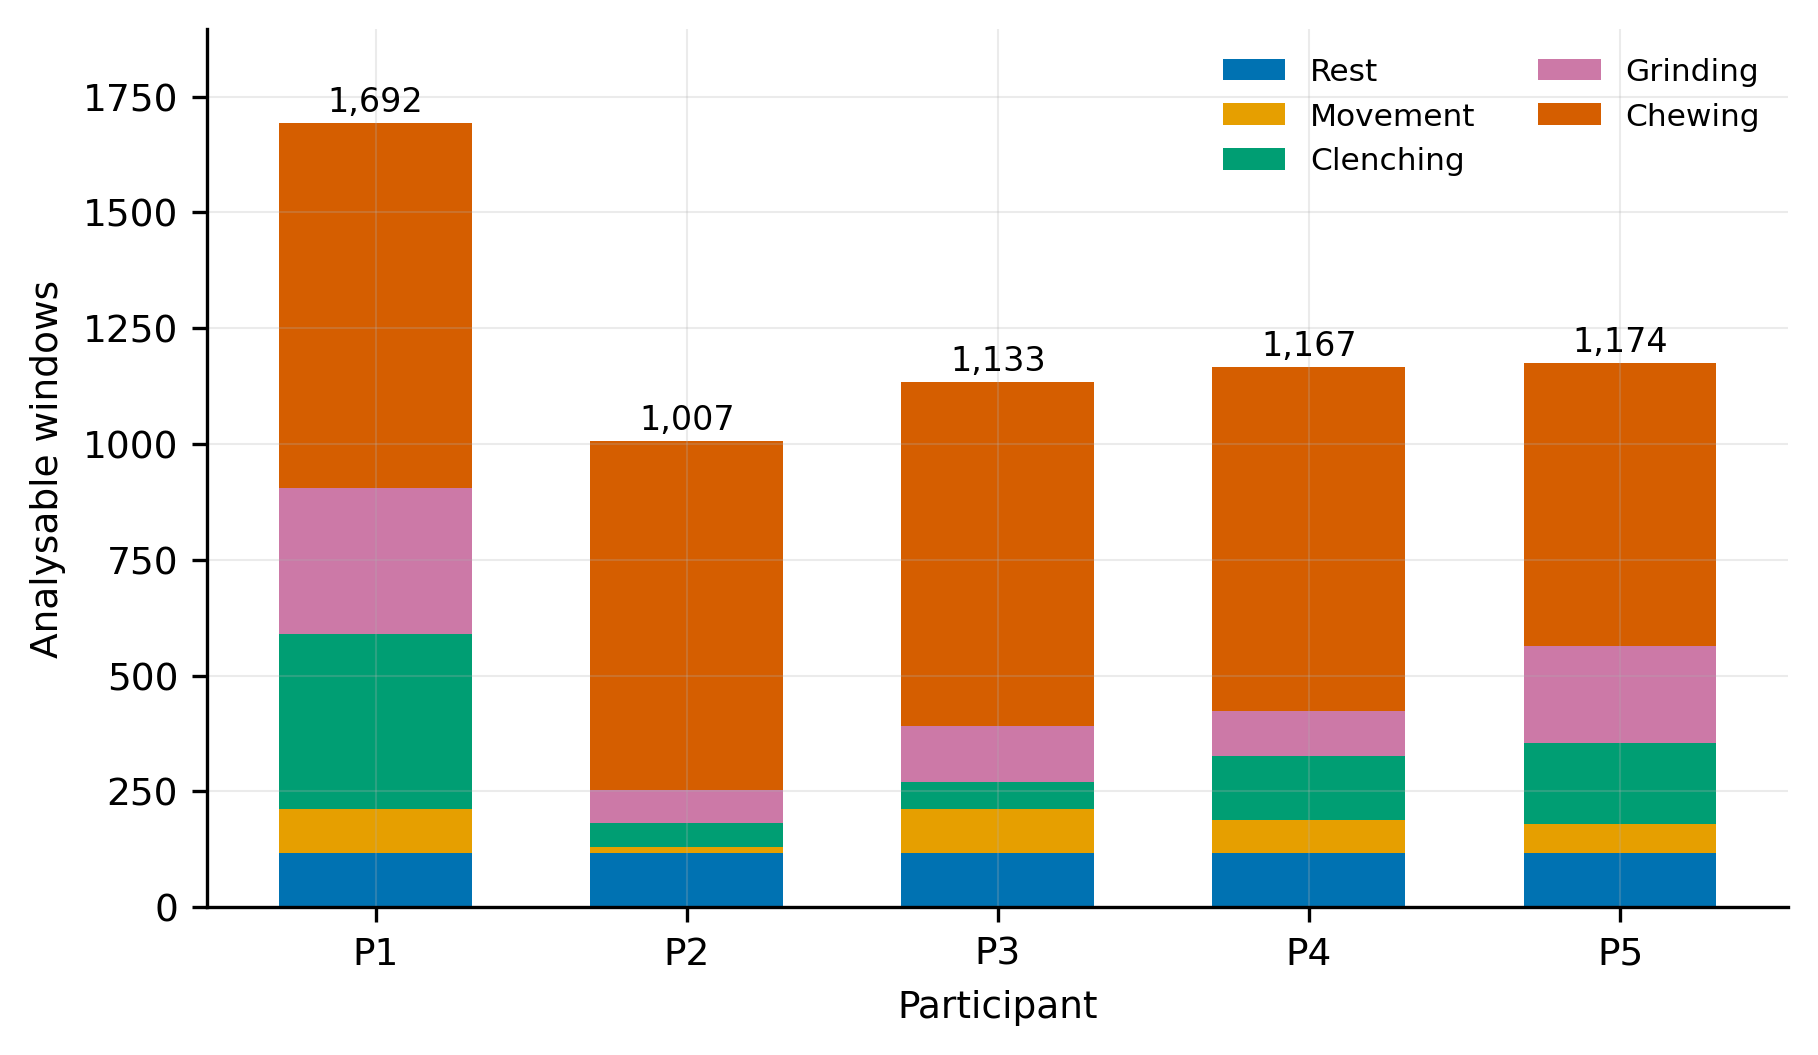
\includegraphics[width=0.78\linewidth]{Figures/sample_flow.png}
  \caption{Analyzable windows per participant and class after the containment, transition-guard and startup-guard exclusions. Participants are labeled P1--P5 here and in every later figure, in the same order as Table~\ref{tab:persubject}. Class sizes are strongly unequal both between classes---chewing supplies 58.9\% of all windows---and between participants within a class, which is why class weighting, minority-only augmentation and participant-level aggregation are all used.}
  \Description{Stacked bar chart of window counts per participant, colored by task family.}
  \label{fig:sample_flow}
\end{figure*}

\subsection{Mains interference and the corrected filter chain}

Every result in this paper was regenerated after a spectral audit of the raw recordings, which is reported here because it changed the analysis substantially.

The acquisition software applied its own fixed notch, recorded in every metadata sidecar, and that notch removed the 60-Hz fundamental before the data were written to disk. Interference survived at the harmonics instead. Measured against the local noise floor of the raw signals, the peaks at 180, 300, and 420~Hz ranged from tens of times that floor in the least affected participant to more than a million times it in the most affected. Across all 100 recordings, 62 had more than 30\% of their raw in-band EMG power concentrated within $\pm 3$~Hz of a mains multiple, and in the five dedicated quiet-rest recordings that share was 91.3--99.8\%.

The preprocessing chain used in earlier analyses of this dataset was a single 60-Hz notch ($Q=30$) followed by the 20--450-Hz band-pass. On the recordings described above it removed the only mains frequency that was already absent and passed every frequency that was present: the mains share of in-band power after filtering was 91.4--99.8\%, essentially unchanged from the raw signal (Fig.~\ref{fig:filter_fix}a, c). A filter-response plot of that chain looks entirely conventional, which is why the problem was not visible until the response was drawn over the measured spectrum of the data.

The corrected chain notches every mains multiple inside the pass band---60, 120, 180, 240, 300, 360, and 420~Hz---before the same fourth-order Butterworth band-pass from 20 to 450~Hz. Each notch is \emph{constant-width} (8~Hz at $-3$~dB, so $Q = f_0/8$) rather than constant-$Q$. Constant $Q$ would give a 2-Hz notch at 60~Hz and a 14-Hz notch at 420~Hz, that is, the narrowest response exactly where the hardware notch left a residue and the widest where nothing survives. Both variants remove 56~Hz of the 430-Hz pass band, an identical 13\% cost, but at that same cost the constant-width bank left the worst-contaminated cell at $3.2\times$ its local noise floor against $25.6\times$ for constant $Q$, an eight-fold reduction in residual interference. After correction, the mains share of in-band power in the quiet-rest recordings fell to 0.46--0.66\% (Fig.~\ref{fig:filter_fix}b, c). A comb filter and spectral interpolation were also implemented and measured on the same windows; both left more residual interference, and spectral interpolation is additionally acausal by construction. The filter chain was chosen on this interference criterion, which can be specified in advance, and not on held-out classification score.

The microphone signal received a second-order 20-Hz high-pass to remove its large DC offset. No further spectral shaping was applied, because the transducer's frequency response is undocumented. The 5-Hz high-pass stage described in the earlier version of this pipeline followed a 20--450-Hz band-pass and was therefore a no-op; it was removed rather than carried forward.

All filtering is zero-phase (forward--backward second-order sections), applied to the whole continuous recording before any window is cut. Zero-phase filtering reads samples from the future of each output sample. It is appropriate for the offline analysis reported here and it cannot support a streaming, wearable, or real-time claim; a causal mode exists in the implementation and the mode used is recorded in every run bundle.

\begin{figure*}[t]
  \centering
  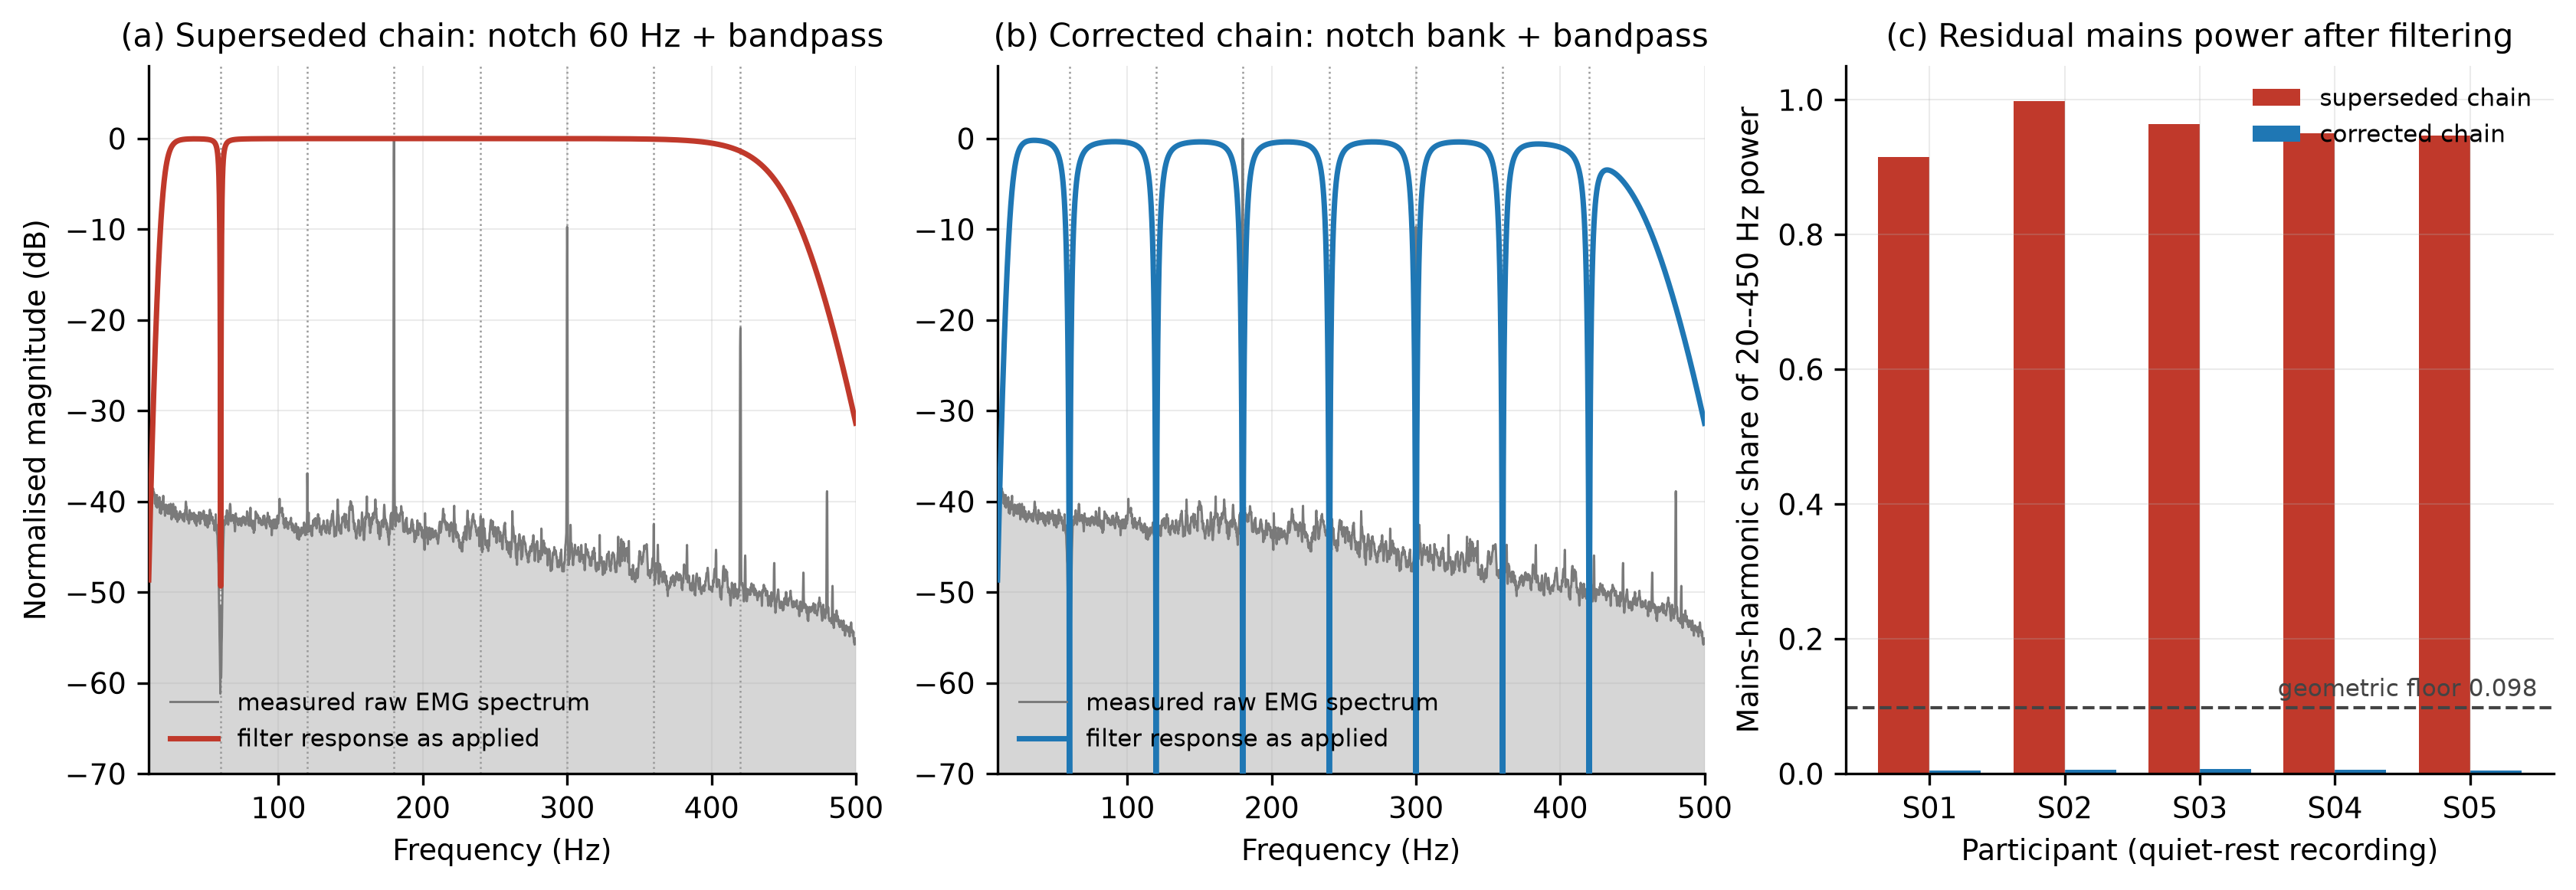
\includegraphics[width=\linewidth]{Figures/filter_defect_and_correction.png}
  \caption{The mains-harmonic defect and its correction. (a) The superseded chain: the 60-Hz notch lands where the acquisition hardware had already removed the fundamental, while the tall harmonic peaks at 180, 300 and 420~Hz pass through the band-pass untouched. (b) The corrected chain: seven constant-width notches land on the peaks. Gray traces are the mean raw EMG spectrum of the five dedicated quiet-rest recordings; colored traces are the zero-phase response as actually applied; dotted lines mark 60~Hz and its harmonics. (c) Share of 20--450-Hz power lying within $\pm3$~Hz of a mains multiple, per participant, after each chain. The dashed line marks the 0.098 share a perfectly white signal would score, because seven $\pm3$-Hz bands occupy 42~Hz of a 430-Hz pass band; a notch bank scores below it by deleting those bins.}
  \Description{Three panels: two filter responses drawn over the measured raw EMG spectrum, and a bar chart of residual mains power per participant.}
  \label{fig:filter_fix}
\end{figure*}

\subsection{Normalization and wavelet decomposition}

EMG and microphone signals were z-scored per channel using means and standard deviations computed \emph{only} from the training participants of the fold in question. The list of participants that produced each fold's statistics is stored with the fold and asserted not to contain the held-out participant before that participant is evaluated. A per-participant (transductive) normalization scope is implemented and prespecified as a separate configuration, but it is not used for any number reported here; the strict scope is the one that would support a deployment claim without a fitting session.

Figure~\ref{fig:emg_preprocessing} shows the chain on a real excerpt. EMG signals were then decomposed using the Daubechies-4 wavelet at four levels, and the EMG sub-branches used $A_4$ ($<38$~Hz), $D_3$ (75--150~Hz), and $D_1$ (300--600~Hz, of which only the 300--450-Hz portion survives the band-pass). Daubechies wavelets were selected because of their compact support and prior use in transient EMG analysis~\cite{englehart2003robust}. Audio signals were decomposed using the Coiflet-5 wavelet at five levels, with sub-branches $A_5$ ($<19$~Hz), $D_3$ (75--150~Hz) and $D_1$ (300--600~Hz), selected in preliminary testing for its time--frequency representation of transient acoustic features~\cite{bharathi2025unveiling}.

\begin{figure*}[h]
  \centering
  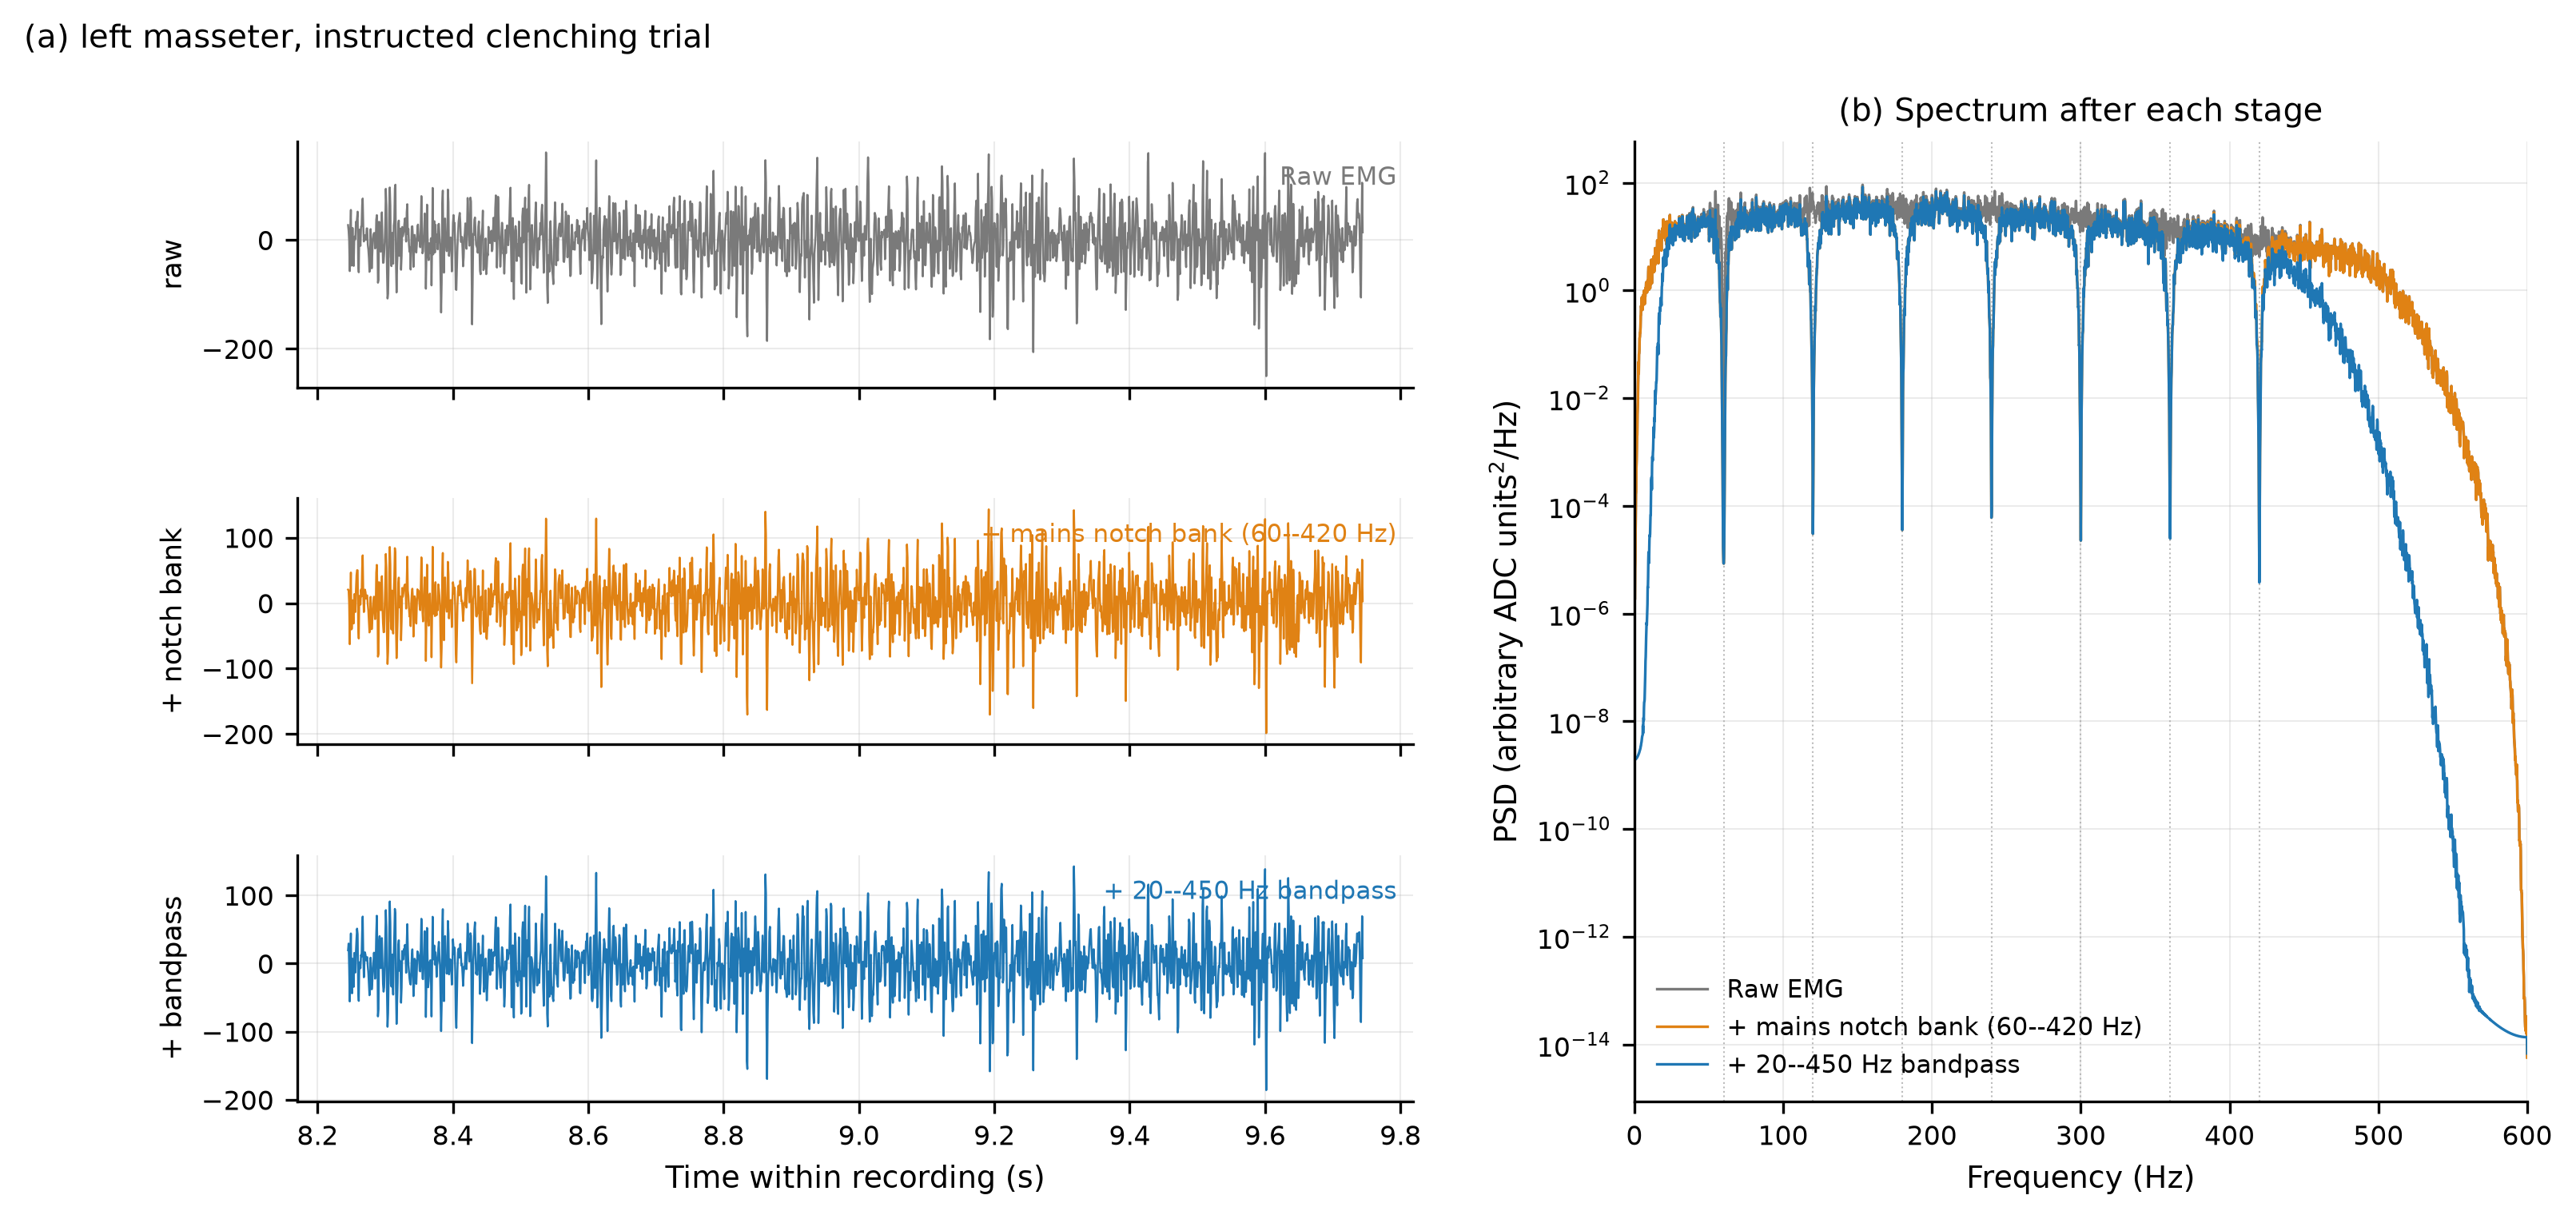
\includegraphics[width=\linewidth]{Figures/preprocessing_stages_5class.png}
  \caption{Production preprocessing on a real excerpt of an instructed clenching trial (left masseter channel). (a) Time domain after each stage. (b) Power spectrum after each stage; the notch bank removes the seven mains multiples marked by dotted lines and the band-pass then removes content outside 20--450~Hz. The chain is applied to the continuous recording and windows are cut afterwards.}
  \label{fig:emg_preprocessing}
\end{figure*}

\subsection{Model architecture}

The model processed EMG and audio in separate branches before fusion (Fig.~\ref{fig:architecture}). The EMG branch contained three CNN sub-branches, one per retained wavelet band. Each sub-branch applied a 3-tap convolution to 8 channels, batch normalization, a rectified linear unit, max pooling by 2, a second 3-tap convolution to 16 channels, batch normalization, a rectified linear unit, and adaptive average pooling to a single value per channel, contributing 16 features per band and 48 EMG features in total. The audio branch used an analogous structure with 4 and 8 channels and produced 24 features.

The 72 concatenated features were passed to a fusion multilayer perceptron (MLP) with dimensions $72\rightarrow48\rightarrow32$. Batch normalization, a rectified linear unit, and dropout with probability 0.5 were applied in each hidden layer. A final linear layer produced logits for rest, movement, clenching, grinding, and chewing. The complete model has 7,485 trainable parameters (1,656 in the EMG branch, 432 in the audio branch, 5,232 in the fusion MLP, and 165 in the classification head), or 29.2~KiB at 32-bit precision. In the modality ablations the unused branch is not constructed at all, so its parameters are genuinely removed rather than fed zeros.

\begin{figure*}[t]
  \centering
  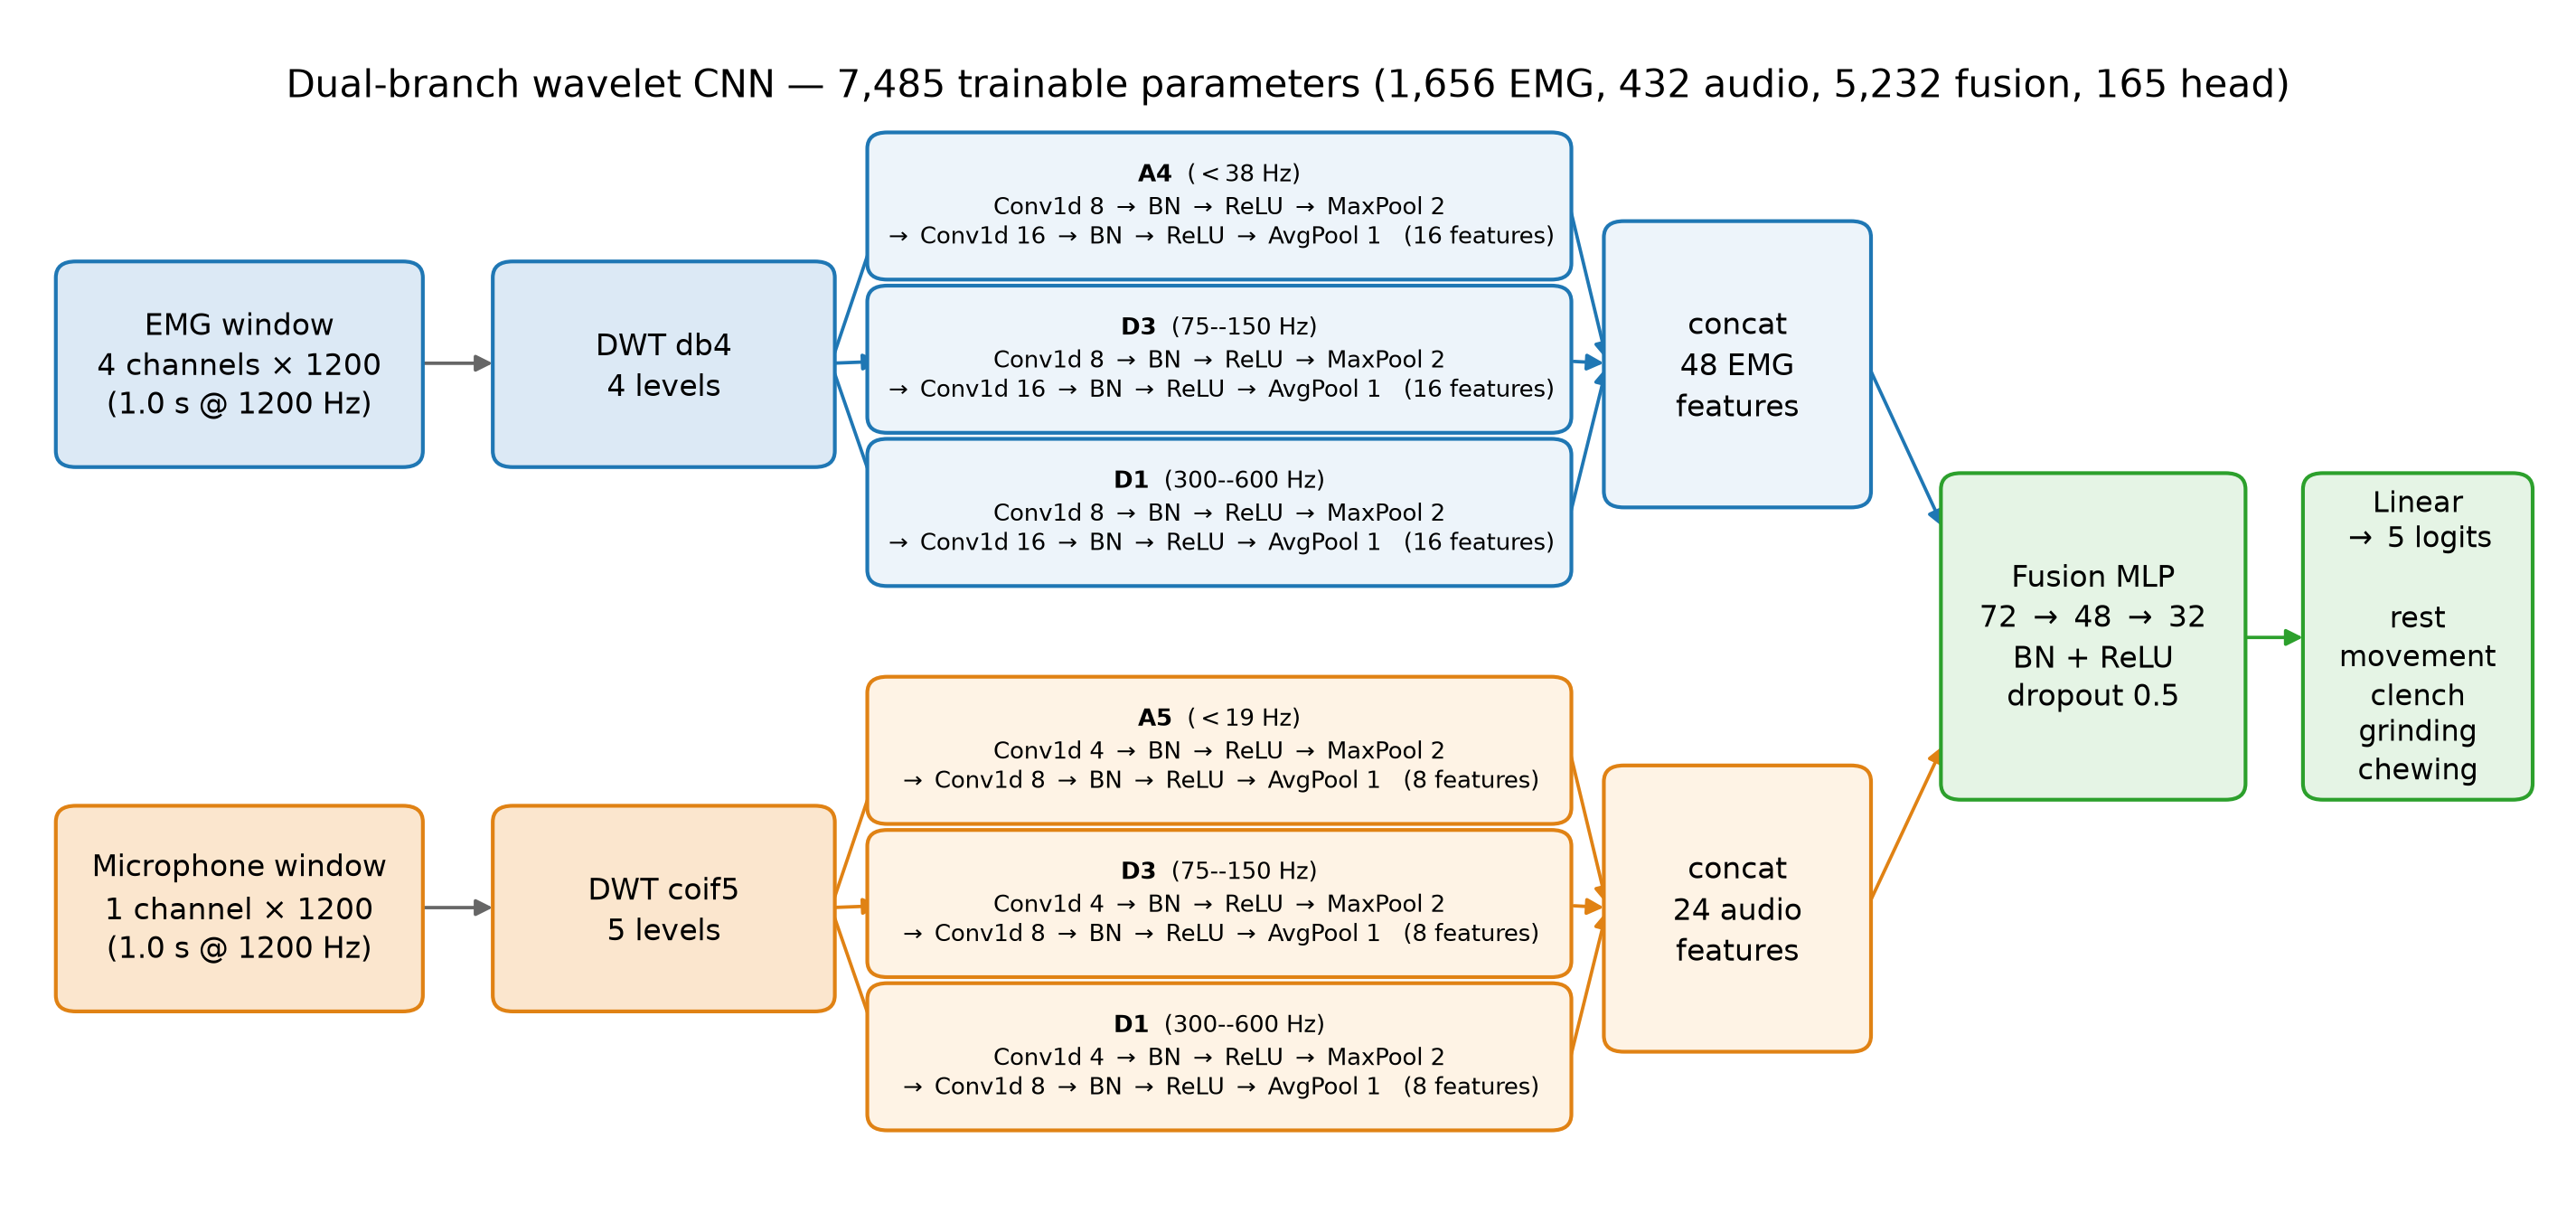
\includegraphics[width=\linewidth]{Figures/pipeline_5class.png}
  \caption{Dual-branch five-class architecture. EMG and audio undergo modality-specific wavelet decomposition before processing by parallel per-band CNN sub-branches. Extracted features are concatenated and classified by a fusion MLP with outputs for rest, movement, clenching, grinding, and chewing. Layer widths, wavelet families, band edges and parameter counts are read from the instantiated model.}
  \Description{Separate EMG and audio wavelet-CNN pathways merge in a five-output fusion multilayer perceptron.}
  \label{fig:architecture}
\end{figure*}

\subsection{Training and evaluation}

To address class imbalance after adding rest, the model used inverse-frequency class weights recomputed within each outer training fold, and augmentation of minority-class training windows by amplitude scaling in $[0.9, 1.1]$ (applied with probability 0.5), additive Gaussian noise at 2\% of the window standard deviation (probability 0.3), and circular shifts of up to $\pm50$ samples (probability 0.3). A window was eligible for augmentation with probability 0.4 and only if its class fell below 70\% of the largest class in that fold, so chewing windows were never augmented and rest windows were. Augmentation was applied only within the training partition of each fold, enforced structurally: the augmenter raises an error for any stage other than training, and each transformation is seeded by the triple (run seed, epoch, sample identifier) so that it does not depend on worker count or batch order.

Optimization used AdamW with weight decay $1\times10^{-4}$, gradient clipping at norm 1.0, and batch size 64. The loss function and learning rate were selected inside each fold (below) from focal loss~\cite{lin2017focal} with focusing parameter $\gamma = 1.5$ or cross-entropy, and from $3\times10^{-4}$ or $1\times10^{-3}$. Table~\ref{tab:hyperparameters} lists these settings together with the prespecified configurations of the architecture comparison.

Evaluation used \emph{nested} leave-one-subject-out (LOSO). In each of the five outer folds, one participant was sealed as the test set and the remaining four entered a participant-grouped inner LOSO loop of four inner folds. Every normalization statistic, class weight, augmentation minority set and hyperparameter was fitted on inner-training participants only. The best epoch was recorded per inner fold by validation macro-F1, and the epoch budget for the final refit was the median of those best epochs. The model was then refit on all four outer-training participants for exactly that many epochs, with no early stopping and no validation set, and the held-out participant was evaluated exactly once. This is 17 model fits per outer fold ($4$ trials $\times\ 4$ inner folds, plus the refit). The held-out participant's sample identifiers are stored privately and released only by an explicit single-use call, so selection code cannot reach them even accidentally. Macro-F1 was the selection objective rather than accuracy, because accuracy is dominated by chewing. The whole protocol was run with three random seeds, all of which completed all five outer folds, and metrics are computed independently per seed and then summarized. Probabilities are never averaged across seeds and no seed is selected as best.

Across the fifteen fold--seed combinations, the inner loop selected a learning rate of $1\times10^{-3}$ every time and divided almost evenly between cross-entropy (8) and focal loss (7); the epoch budget ranged from 12 to 43 with a median of 26. Each outer fold, including its inner search, took approximately 20 minutes on the training hardware, and the complete run took 5.0 hours.

\textbf{Participant-level metrics are primary.} Accuracy, balanced accuracy, macro precision, recall, F1 and one-vs-rest ROC--AUC are computed within each held-out participant and then summarized across the five participants; all five individual values are reported. Pooled-window metrics are also reported, but only as descriptive summaries, because windows within a participant and recording are correlated. AUC was computed from the saved held-out class probabilities, never from hard labels or a confusion matrix. A class absent from a fold receives no AUC rather than an imputed value. No window-level bootstrap intervals or $p$-values are reported: the windows are clustered and overlapping, and with five participants such tests would overstate precision without supporting a population-level claim. Held-out probabilities are uncalibrated (expected calibration error 0.046); they must not be read as probabilities, but every AUC remains valid because AUC is rank-based and unaffected by any monotone rescaling.

Two secondary analyses were computed post hoc from the same held-out five-class predictions and are labeled as such. First, chewing windows were removed and the four remaining probabilities renormalized, giving a four-class problem over rest, movement, clenching, and grinding. Second, predictions and probabilities were collapsed into instructed clenching/grinding versus rest/movement/chewing. Both re-read one model rather than training a new one; separately trained versions of these tasks are prespecified but were not part of this run. The second analysis provides a binary comparison against quiet rest and other instructed activities, but it is still not a clinical bruxism-detection analysis because the positive tasks were elicited and the background class does not include unrestricted free-living behavior.

\begin{table}[h]
  \caption{Hyperparameters. Values for the dual-branch CNN are those of the reported run; the loss and learning rate were selected inside each fold from the stated search space. The remaining rows describe the prespecified configurations of the architecture comparison, which has not yet been run on the corrected signal. Those three models receive the identical EMG and audio pair and a fixed training configuration (AdamW, $10^{-3}$, focal loss with $\gamma=1.5$, batch size 64, balanced class weights), so the comparison isolates the architecture.}
  \label{tab:hyperparameters}
  \centering
  \footnotesize
  \begin{tabular*}{\columnwidth}{@{\extracolsep{\fill}}lll@{}}
    \toprule
    Method & Hyperparameter & Value \\
    \midrule
    \multirow{9}{*}{\shortstack[l]{Wavelet dual-\\branch CNN}}
      & Optimizer & AdamW \\
      & LR search space & $\{3, 10\}\times10^{-4}$ \\
      & LR selected & $10^{-3}$ (15/15) \\
      & Weight decay & $1\times10^{-4}$ \\
      & Dropout & 0.5 \\
      & Batch size & 64 \\
      & Loss search space & focal, cross-entropy \\
      & Focal-loss $\gamma$ & 1.5 \\
      & Epoch budget & Median inner best \\
    \midrule
    \multirow{4}{*}{\shortstack[l]{Dual-branch\\temporal CNN}}
      & Wavelet front end & As above \\
      & Pooling per band & Mean, SD, max \\
      & Modulation spectrum & 6 bins \\
      & Dropout & 0.5 \\
    \midrule
    \multirow{4}{*}{\shortstack[l]{Early-fusion\\CNN (raw)}}
      & Conv.\ channels & 16, 32, 64 \\
      & Kernel size & 7 \\
      & Pool size & 4 \\
      & Dropout & 0.5 \\
    \midrule
    \multirow{4}{*}{\shortstack[l]{Bidirectional\\LSTM}}
      & Hidden dimensions & 32 \\
      & Number of layers & 1 \\
      & Input decimation & $8\times$ \\
      & Dropout & 0.5 \\
    \bottomrule
  \end{tabular*}
\end{table}

\section{Results}

All results below come from one nested-LOSO run of the fused dual-branch wavelet CNN on the corrected signal (five outer folds $\times$ three seeds; 6,173 held-out window predictions per seed, 18,519 in total). Every value was recomputed from the saved prediction ledger. Results obtained before the filter correction are superseded and are not restated for comparison.

\subsection{Five-class performance}

Averaged over the five held-out participants, the fused model achieved 82.1\% accuracy, 79.1\% balanced accuracy, 73.6\% macro-F1, and a macro one-vs-rest ROC--AUC of 0.962 (Table~\ref{tab:results}). The three seeds agreed closely (accuracy 81.1\%, 82.8\% and 82.2\%; macro-F1 71.7\%, 74.6\% and 74.5\%; macro AUC 0.960, 0.963 and 0.963), so seed-to-seed variation is small relative to the variation between participants. Pooling held-out windows across participants instead---a descriptive summary only, because the windows are correlated---gives 81.0\% accuracy, 70.5\% macro precision, 77.9\% macro recall, 72.3\% macro-F1 and a macro AUC of 0.942.

For the newly added rest class, the fused model achieved 74.4\% precision, 92.5\% recall, an F1 of 82.2\%, and a one-vs-rest AUC of 0.960 (Table~\ref{tab:perclass}). Rest is therefore the second-best-separated class after chewing, and the best-recalled class of the five, which is the outcome the class was added to test: activity windows can now be scored against a quiet non-event condition rather than only against one another.

The baseline comparison specified for RQ3---the dual-branch temporal CNN, an early-fusion CNN on the raw signals, and a bidirectional LSTM, all receiving the identical EMG and audio pair---has not been run since the filter correction, and the earlier numbers were measured through the defective chain, in which mains harmonics carried the majority of the in-band power. They are therefore withdrawn rather than reproduced, and Table~\ref{tab:results} marks those rows as pending. The only comparison currently available on the corrected signal comes from a screening harness that fits one model per outer fold on 35 band-energy features, with no nested hyperparameter selection and a feature set chosen after seeing these five participants: it is directionally informative and optimistic in level. On identical windows and folds it reached 0.679 macro-F1 / 79.7\% accuracy for logistic regression and 0.646 / 77.7\% for gradient boosting. Both sit below the network's 0.736 participant-level macro-F1, but the comparison is not like-for-like and does not settle RQ3 in either direction.

The modality ablation specified for RQ2 is pending for the same reason, and Table~\ref{tab:modality_ablation} therefore carries the fused row alone. The matched conditions---fusion, EMG only and audio only, each on the five-class task and on the same task with chewing removed---are prespecified and share identical windows, folds, seeds and epoch budgets, so the contrast will isolate the modality when that run completes.

\begin{table*}[t]
  \centering
  \caption{Five-class performance, averaged over the five held-out participants and three seeds. Classes are rest, movement, clenching, grinding, and chewing. Values describe this five-participant dataset and are not population-level superiority tests. Baseline rows await the confirmatory sweep on the corrected signal; the screening rows come from a single-fit harness and are reported for direction only.}
  \label{tab:results}
  \small
  \begin{tabular}{lccccc}
    \toprule
    Method & Accuracy & Macro prec. & Macro rec. & Macro F1 & Macro AUC \\
    \midrule
    \textbf{Wavelet dual-branch CNN (fusion)} & \textbf{82.1\%} & \textbf{70.5\%} & \textbf{77.9\%} & \textbf{73.6\%} & \textbf{0.962} \\
    \midrule
    Logistic regression, band energies$^{a}$ & 79.7\% & -- & -- & 67.9\% & -- \\
    Gradient boosting, band energies$^{a}$ & 77.7\% & -- & -- & 64.6\% & -- \\
    \midrule
    Dual-branch temporal CNN & \multicolumn{5}{c}{\emph{pending re-measurement}} \\
    Early-fusion CNN, raw signals & \multicolumn{5}{c}{\emph{pending re-measurement}} \\
    Bidirectional LSTM & \multicolumn{5}{c}{\emph{pending re-measurement}} \\
    \bottomrule
  \end{tabular}
  \begin{flushleft}\footnotesize
  Macro precision and recall for the CNN are pooled-window values; accuracy, macro-F1 and macro AUC are participant-level means.\\
  $^{a}$Screening harness: one model fit per outer fold, no nested hyperparameter selection, feature set chosen after seeing these participants. Optimistic in level and not a confirmatory baseline.
  \end{flushleft}
\end{table*}

\begin{table*}[t]
  \centering
  \caption{Five-class modality ablation. The confirmatory ablation on the corrected signal has not been run; the previously reported audio contribution was measured through the defective filter chain and is withdrawn rather than restated.}
  \label{tab:modality_ablation}
  \small
  \begin{tabular}{lcccccc}
    \toprule
    Configuration & Accuracy & Macro prec. & Macro rec. & Macro F1 & Macro AUC & Acc.\ difference \\
    \midrule
    Audio only & \multicolumn{6}{c}{\emph{pending}} \\
    EMG only & \multicolumn{6}{c}{\emph{pending}} \\
    \textbf{EMG + audio} & 82.1\% & 70.5\% & 77.9\% & 73.6\% & 0.962 & --- \\
    \bottomrule
  \end{tabular}
\end{table*}

\begin{table*}[t]
  \centering
  \caption{Per-class performance of the five-class fused model on held-out windows, averaged over three seeds. AUC is one-vs-rest, computed from held-out probabilities.}
  \label{tab:perclass}
  \small
  \begin{tabular}{lccccc}
    \toprule
    Class & Precision & Recall & F1 & AUC & Windows \\
    \midrule
    Rest & 74.4\% & 92.5\% & 82.2\% & 0.960 & 590 \\
    Movement & 34.9\% & 75.9\% & 47.8\% & 0.934 & 333 \\
    Clenching & 74.3\% & 64.0\% & 68.7\% & 0.921 & 799 \\
    Grinding & 72.1\% & 71.6\% & 71.8\% & 0.920 & 816 \\
    Chewing & 97.0\% & 85.4\% & 90.8\% & 0.974 & 3,635 \\
    \midrule
    \textbf{Macro average} & 70.5\% & 77.9\% & 72.3\% & 0.942 & 6,173 \\
    \bottomrule
  \end{tabular}
\end{table*}

Per-class one-vs-rest ROC and precision--recall curves are shown in Fig.~\ref{fig:roc_pr}. The ordering is consistent across both views: chewing and rest separate well, whereas movement combines a high AUC with a low average precision---0.914 and 0.553 respectively for the seed drawn---reflecting its small support of 333 of 6,173 windows rather than an inability to rank it.

\begin{figure*}[h]
  \centering
  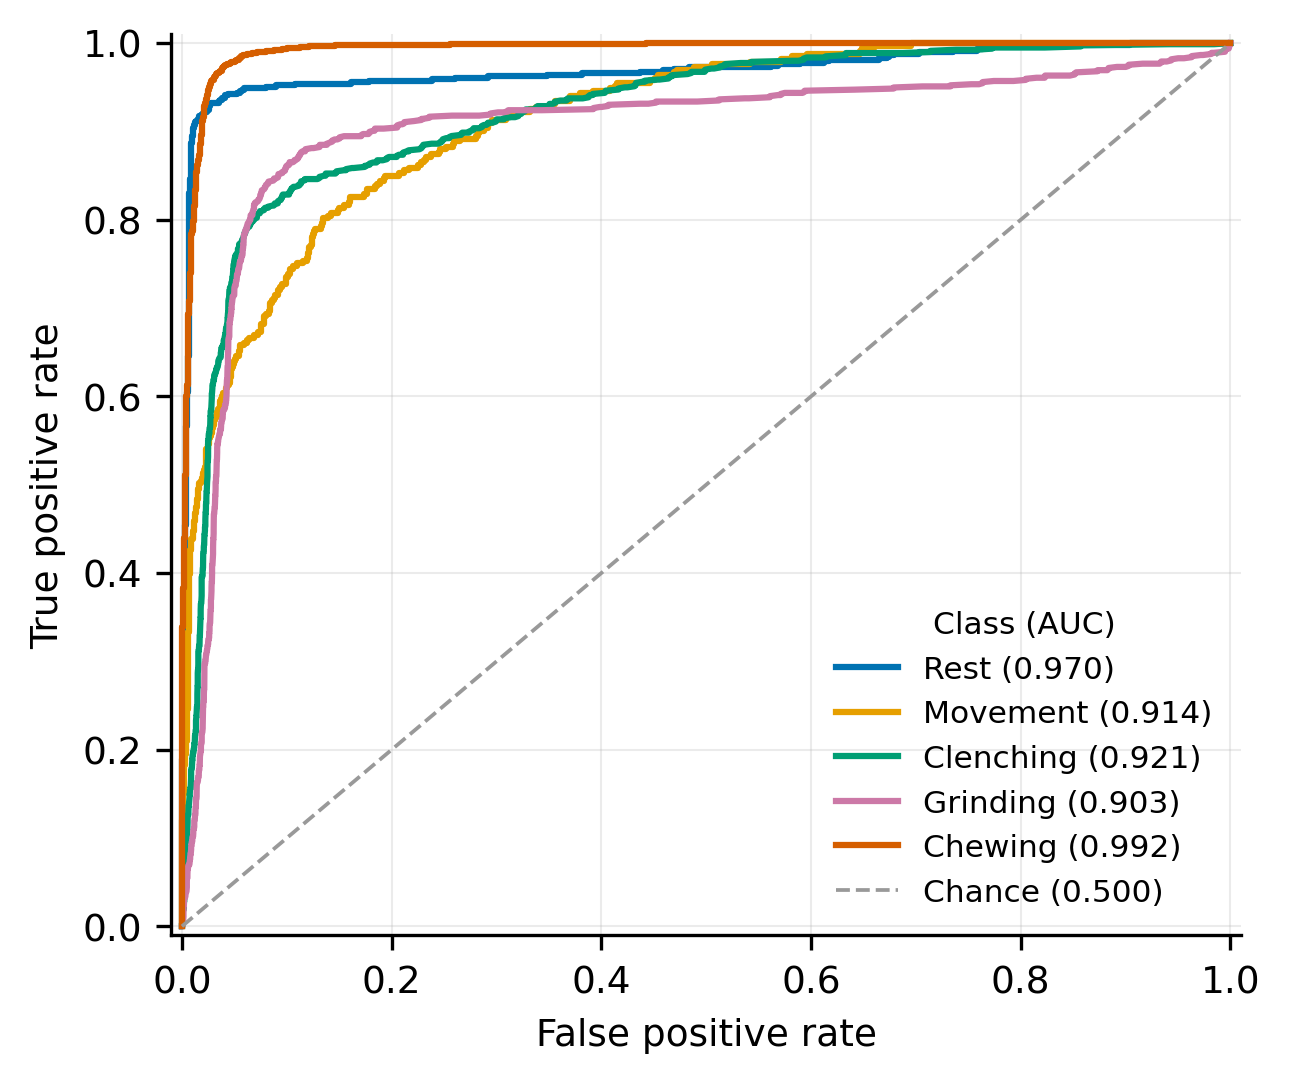
\includegraphics[width=0.49\linewidth]{Figures/five_class_roc_curves.png}
  \hfill
  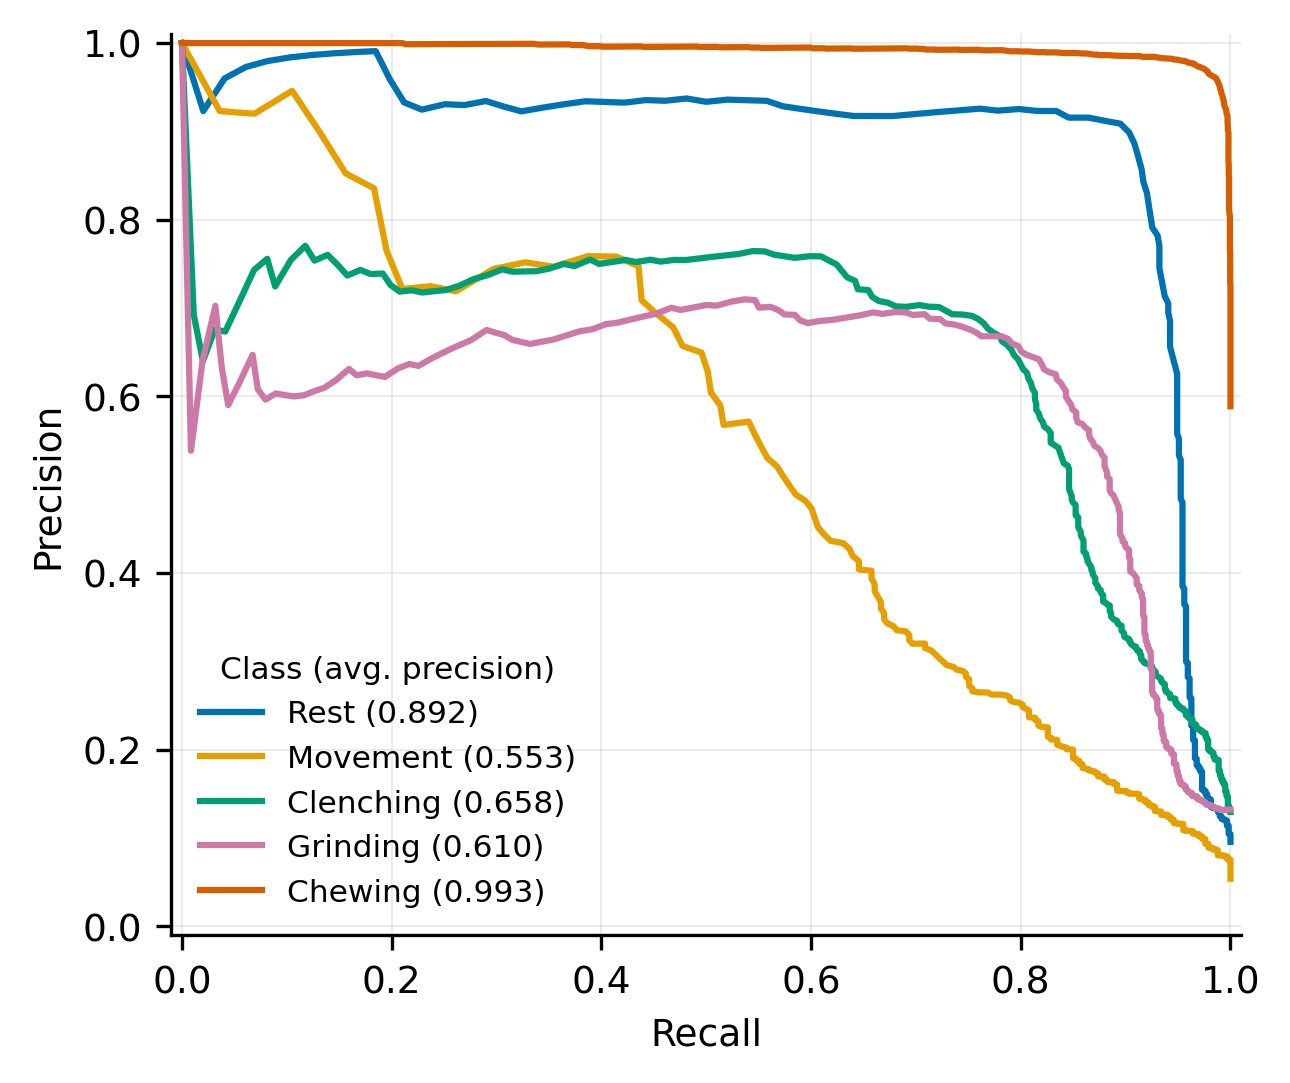
\includegraphics[width=0.49\linewidth]{Figures/five_class_pr_curves.png}
  \caption{One-vs-rest ROC (left) and precision--recall (right) curves for the five experimental classes, pooled over the held-out windows of seed 0 (the lowest seed index, a fixed rule rather than a choice made after seeing the scores). Each curve depicts one trained model per fold, so the legend values are that seed's; the three-seed means are in Table~\ref{tab:perclass}. Precision--recall separates the classes far more sharply than ROC does, because it is sensitive to the very unequal class sizes.}
  \Description{Two panels of per-class ROC and precision-recall curves.}
  \label{fig:roc_pr}
\end{figure*}

\subsection{Secondary analyses with rest}

When chewing was excluded, the remaining four-class problem comprised rest, movement, clenching, and grinding. Averaged over the held-out participants, this analysis yielded 79.8\% accuracy, 77.9\% macro-F1, and a macro AUC of 0.944; the corresponding pooled-window values were 77.1\% accuracy, 76.6\% macro precision, 78.4\% macro recall, 77.2\% macro-F1, and a macro AUC of 0.917 (Table~\ref{tab:sensitivity}). Removing chewing lowers accuracy by 2.3 percentage points but \emph{raises} macro-F1 by 4.3 points, because the metric is no longer dominated by a single large, easily separated class. Reporting both prevents the comparatively recognizable chewing class from carrying the global summary.

For a task-level binary analysis, clenching and grinding were treated as the positive group and rest, movement, and chewing as the comparison group. This yielded 93.6\% accuracy, 90.6\% precision, 84.3\% sensitivity, 96.9\% specificity, an F1 of 87.3\%, and a ROC--AUC of 0.966 on pooled windows, and 94.0\% accuracy with a participant-level macro-F1 of 90.9\% and AUC of 0.977. Within the quiet-rest condition, 6.0\% of rest windows (35 of 590 for one seed and 36 of 590 for each of the other two) were classified as clenching or grinding. This analysis includes a laboratory non-event class but still does not measure spontaneous bruxism detection in a continuous free-living stream: a 6\% per-window false-alarm rate at a 0.5-s decision interval would correspond to roughly 440 false alarms per hour if the background were quiet rest throughout, which is precisely the quantity a deployable detector must report and this design cannot estimate.

\begin{table*}[h]
  \caption{Secondary analyses computed post hoc from the held-out five-class predictions, averaged over three seeds. These re-read one trained model; they are not separately trained tasks.}
  \label{tab:sensitivity}
  \centering
  \begin{tabular}{lcccccc}
    \toprule
    Analysis & Accuracy & Precision & Recall & Specificity & F1 & AUC \\
    \midrule
    Excluding chewing$^{a}$ & 77.1\% & 76.6\% & 78.4\% & -- & 77.2\% & 0.917 \\
    Collapsed binary$^{b}$ & 93.6\% & 90.6\% & 84.3\% & 96.9\% & 87.3\% & 0.966 \\
    \bottomrule
  \end{tabular}
  \begin{flushleft}\footnotesize
  Values are pooled over held-out windows. The corresponding participant-level means are 79.8\% accuracy / 77.9\% macro-F1 / 0.944 AUC when chewing is excluded, and 94.0\% accuracy / 90.9\% macro-F1 / 0.977 AUC for the collapsed binary analysis.\\
  $^{a}$Macro precision, recall, F1, and one-vs-rest AUC across rest, movement, clenching, and grinding, after removing chewing windows and renormalizing the remaining four probabilities.\\
  $^{b}$Instructed clenching/grinding treated as positive; rest/movement/chewing treated as the comparison group. This is task discrimination, not clinical diagnosis.
  \end{flushleft}
\end{table*}

\subsection{Class-level diagnostics}

The highest per-class F1 was observed for chewing (90.8\%) and the lowest for movement (47.8\%). Movement's low F1 is a precision problem rather than a detection problem: its recall is 75.9\% and its one-vs-rest AUC is 0.934, but its precision is 34.9\% because it is the smallest class (333 windows, 5.4\% of the total) and absorbs 10.3\% of the 3,635 chewing windows, which are eleven times more numerous. Clenching and grinding were most often confused with each other: 19.3\% of clenching windows were labeled grinding and 13.5\% of grinding windows were labeled clenching, which together account for the majority of both classes' errors. Rest had the highest recall of any class at 92.5\%, and its dominant error was into grinding (5.9\%). Confusion between quiet rest and the combined instructed clenching/grinding group therefore occurred in 6.0\% of rest windows. These errors matter most, because they approximate false alarms under the limited quiet-rest condition.

We used t-distributed stochastic neighbor embedding (t-SNE)~\cite{vandermaaten2008visualizing} to visualize the 72-dimensional fusion features of held-out windows (Fig.~\ref{fig:tsne}). Chewing occupies several large, well-separated regions, consistent with its high AUC and with food-dependent acoustic and rhythmic structure. Rest forms a small number of tight, compact islands, which is what a low-variance quiet condition should look like. Clenching and instructed grinding interleave repeatedly, forming mixed regions rather than separate territories, and movement windows appear mostly as a scatter along the borders of the larger classes rather than as a territory of their own. The embedding therefore reproduces the two error patterns visible in the confusion matrix. Because t-SNE is an exploratory nonlinear visualization whose apparent distances are not metric, these clusters are not evidence of clinical phenotypes and no quantitative claim rests on them.

\begin{figure*}[h]
  \centering
  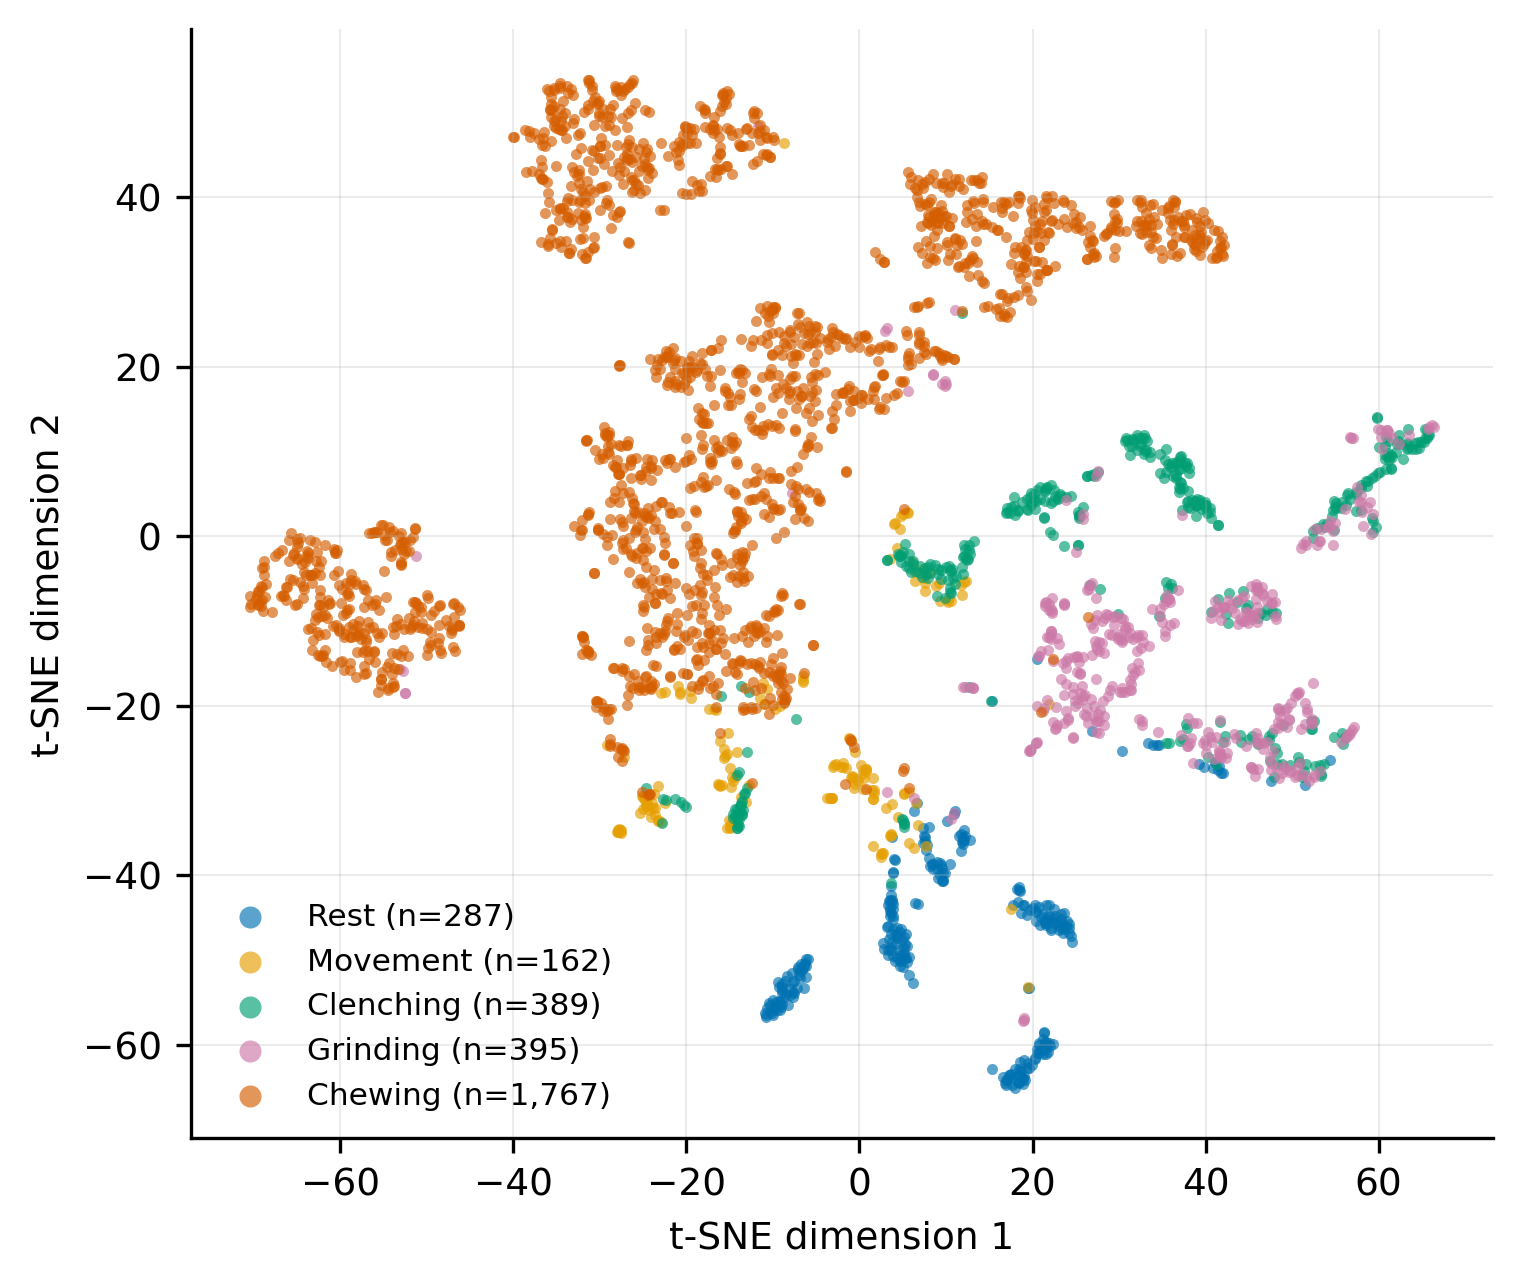
\includegraphics[width=0.72\linewidth]{Figures/tsne_5class.png}
  \caption{t-SNE visualization of the 72-dimensional learned fusion features for held-out windows, colored by experimental class. Chewing occupies large separate regions and rest forms tight compact islands, whereas clenching and instructed grinding interleave and movement scatters along class borders. Embeddings were recomputed from the saved fold checkpoints using only outer-test windows. This exploratory visualization does not establish clinical phenotypes.}
  \Description{Two-dimensional scatter plot of held-out windows colored by the five experimental classes.}
  \label{fig:tsne}
\end{figure*}

The held-out confusion matrix is shown in Fig.~\ref{fig:confusion}. For the seed shown, the diagonal counts were 549 of 590 rest windows, 235 of 333 movement, 531 of 799 clenching, 553 of 816 grinding, and 3,110 of 3,635 chewing. The corresponding class supports are listed in Table~\ref{tab:perclass}.

\begin{figure*}[h]
  \centering
  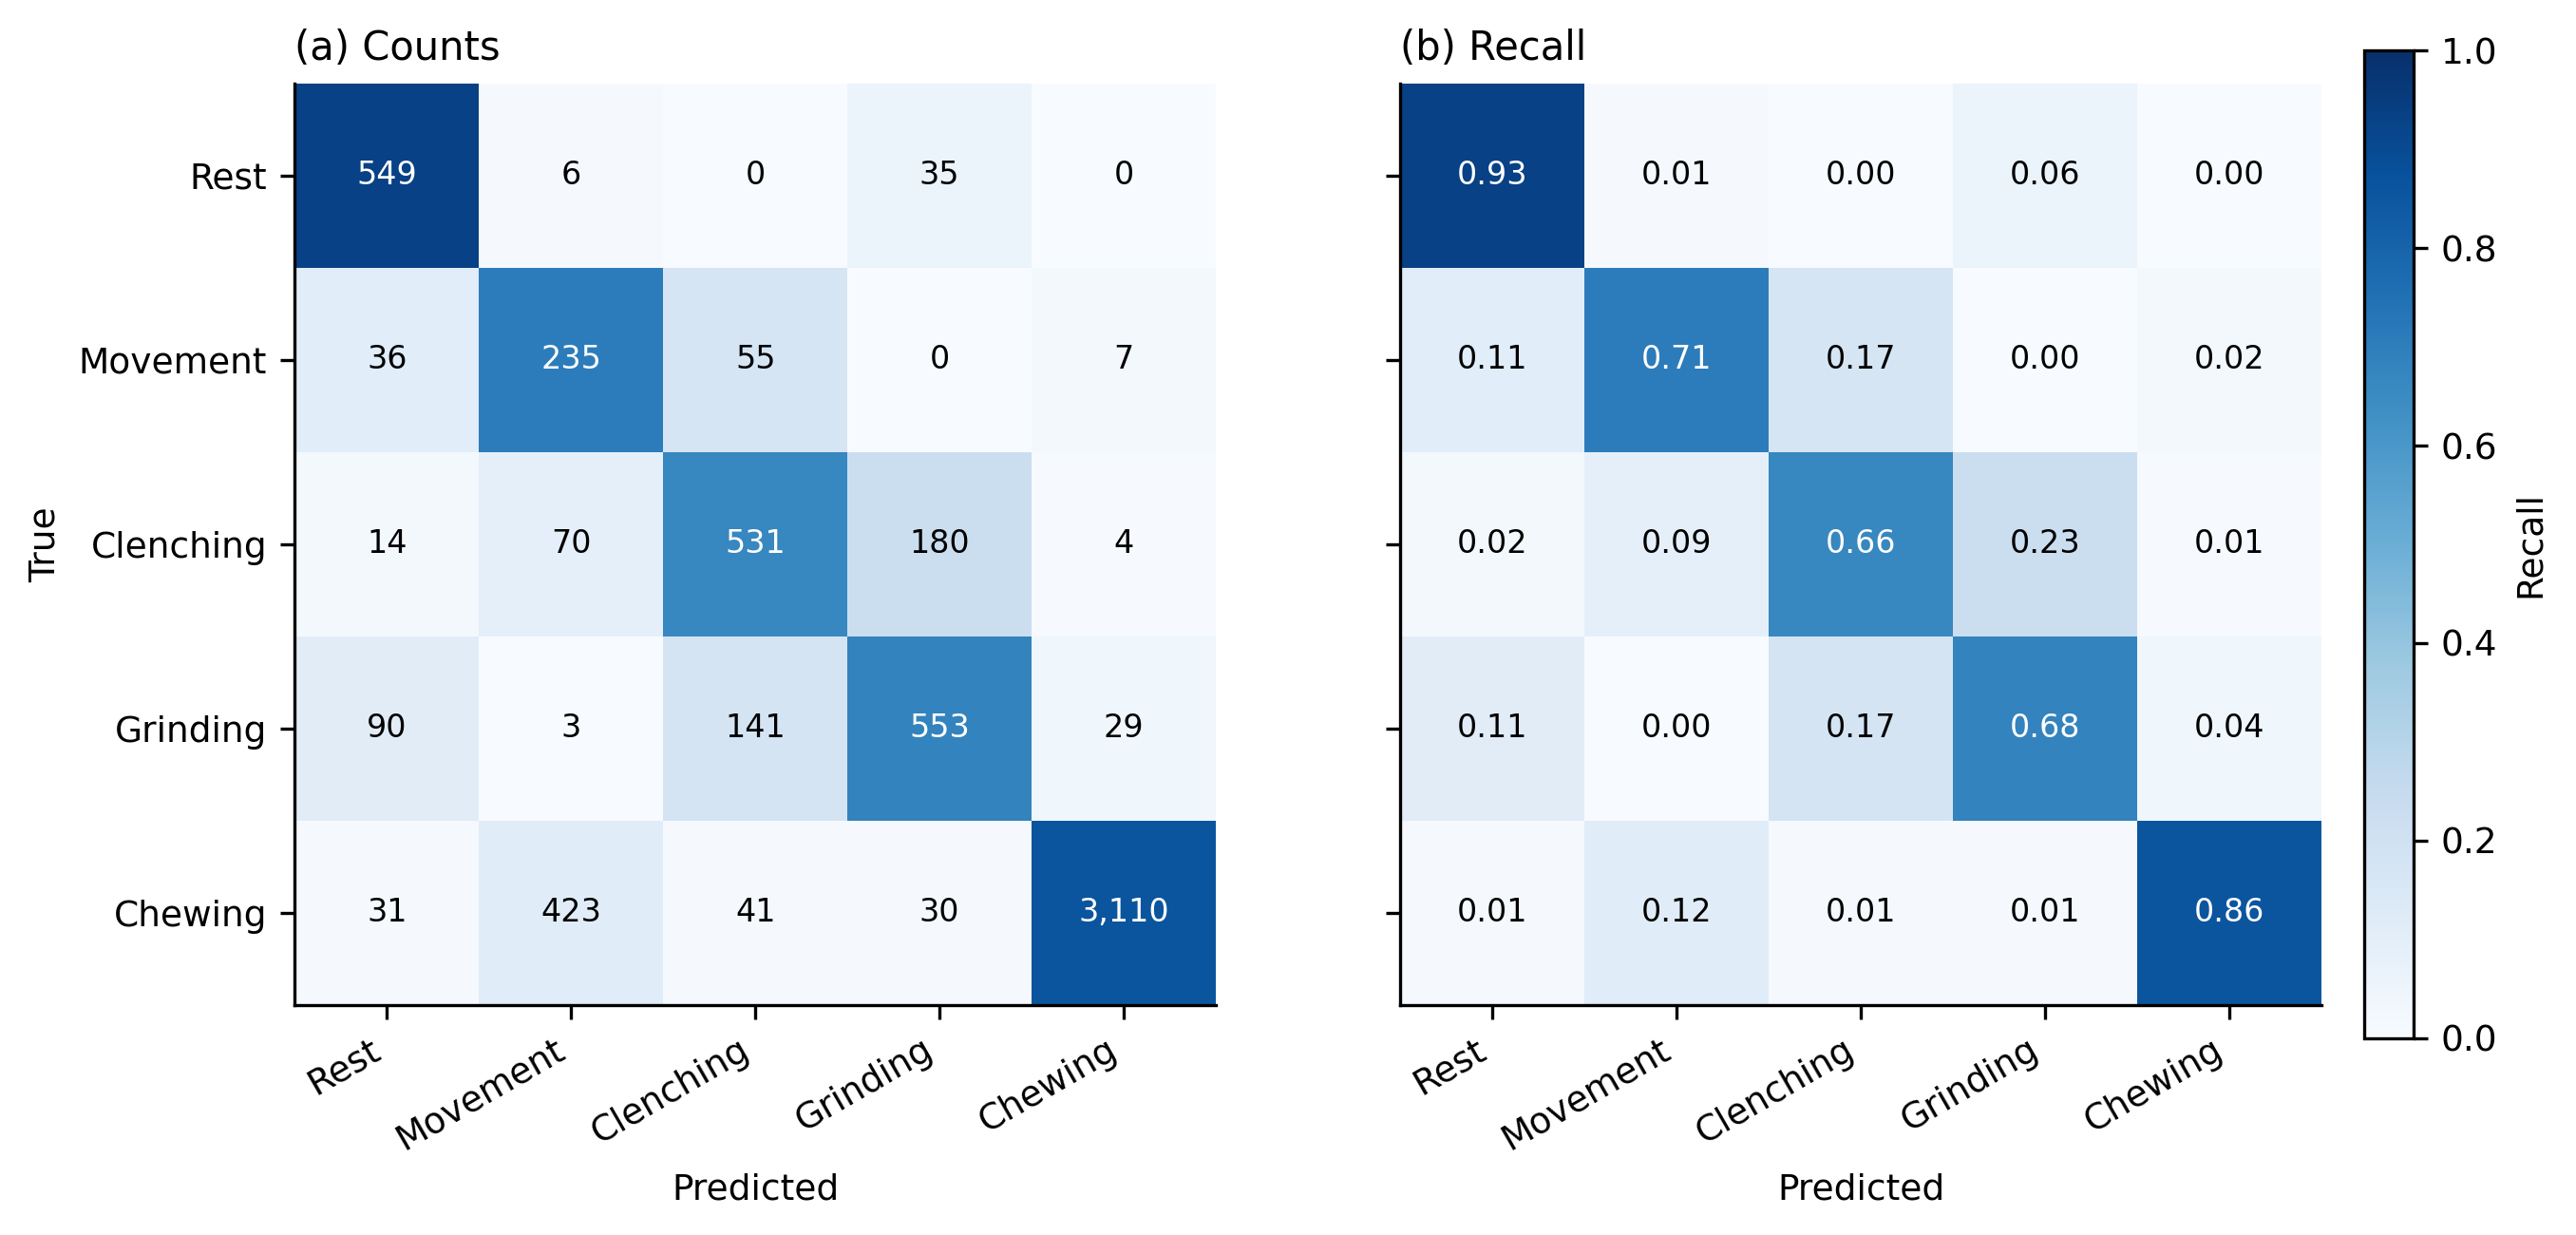
\includegraphics[width=\linewidth]{Figures/confmatrx_5class.png}
  \caption{Held-out confusion matrix for rest, movement, clenching, grinding, and chewing, pooled across the five leave-one-subject-out folds of seed 0 (selected by the fixed lowest-seed-index rule, not by score). (a) Counts. (b) Row-normalized recall. The two dominant error patterns are the mutual clenching--grinding confusion and the leakage of chewing windows into the much smaller movement class.}
  \Description{A five-by-five confusion matrix shown as counts and as row-normalized recall.}
  \label{fig:confusion}
\end{figure*}

\subsection{Participant-level results}

Table~\ref{tab:persubject} reports five-class results for each held-out participant. Across participants, accuracy ranged from 72.0\% to 91.7\%, macro-F1 from 64.5\% to 82.6\%, and macro AUC from 0.896 to 0.985 (Fig.~\ref{fig:per_participant}). The spread is substantial relative to the mean and is not explained by class balance alone.

Two participants illustrate why accuracy and AUC should be read together. Participant 4 had the lowest accuracy (72.0\%) but the second-highest macro AUC (0.982): its held-out windows are ranked well by the model's scores, and the loss is concentrated in where the decision boundaries fall for that participant rather than in the model's ability to order its windows. Participant 1 shows the opposite pattern---the lowest AUC (0.896) and the lowest macro-F1 (64.5\%), at an accuracy no better than participant 4's---and it also contributes the largest single share of windows (1,692 of 6,173), so it dominates any pooled-window summary while counting as one of five in the participant-level summary. This is one concrete reason the participant-level aggregation is treated as primary here.

These five values describe internal LOSO behavior only. They do not estimate performance across age groups, anatomical variation, dentition, bruxism phenotypes, or clinical settings, and with five participants the standard deviations below describe the sample rather than a sampling distribution.

\begin{table}[h]
  \caption{Five-class performance for each held-out participant, averaged over three seeds.}
  \label{tab:persubject}
  \centering
  \footnotesize
  \begin{tabular*}{\columnwidth}{@{\extracolsep{\fill}}lrrrr@{}}
    \toprule
    Held out & $n$ & Acc. & Macro F1 & Macro AUC \\
    \midrule
    Participant 1 & 1,692 & 72.7\% & 64.5\% & 0.896 \\
    Participant 2 & 1,007 & 91.7\% & 74.4\% & 0.977 \\
    Participant 3 & 1,133 & 86.1\% & 74.7\% & 0.971 \\
    Participant 4 & 1,167 & 72.0\% & 71.8\% & 0.982 \\
    Participant 5 & 1,174 & 87.8\% & 82.6\% & 0.985 \\
    \midrule
    Mean & 6,173 & 82.1\% & 73.6\% & 0.962 \\
    SD & --- & 9.1 & 6.5 & 0.037 \\
    \bottomrule
  \end{tabular*}
\end{table}

\begin{figure*}[h]
  \centering
  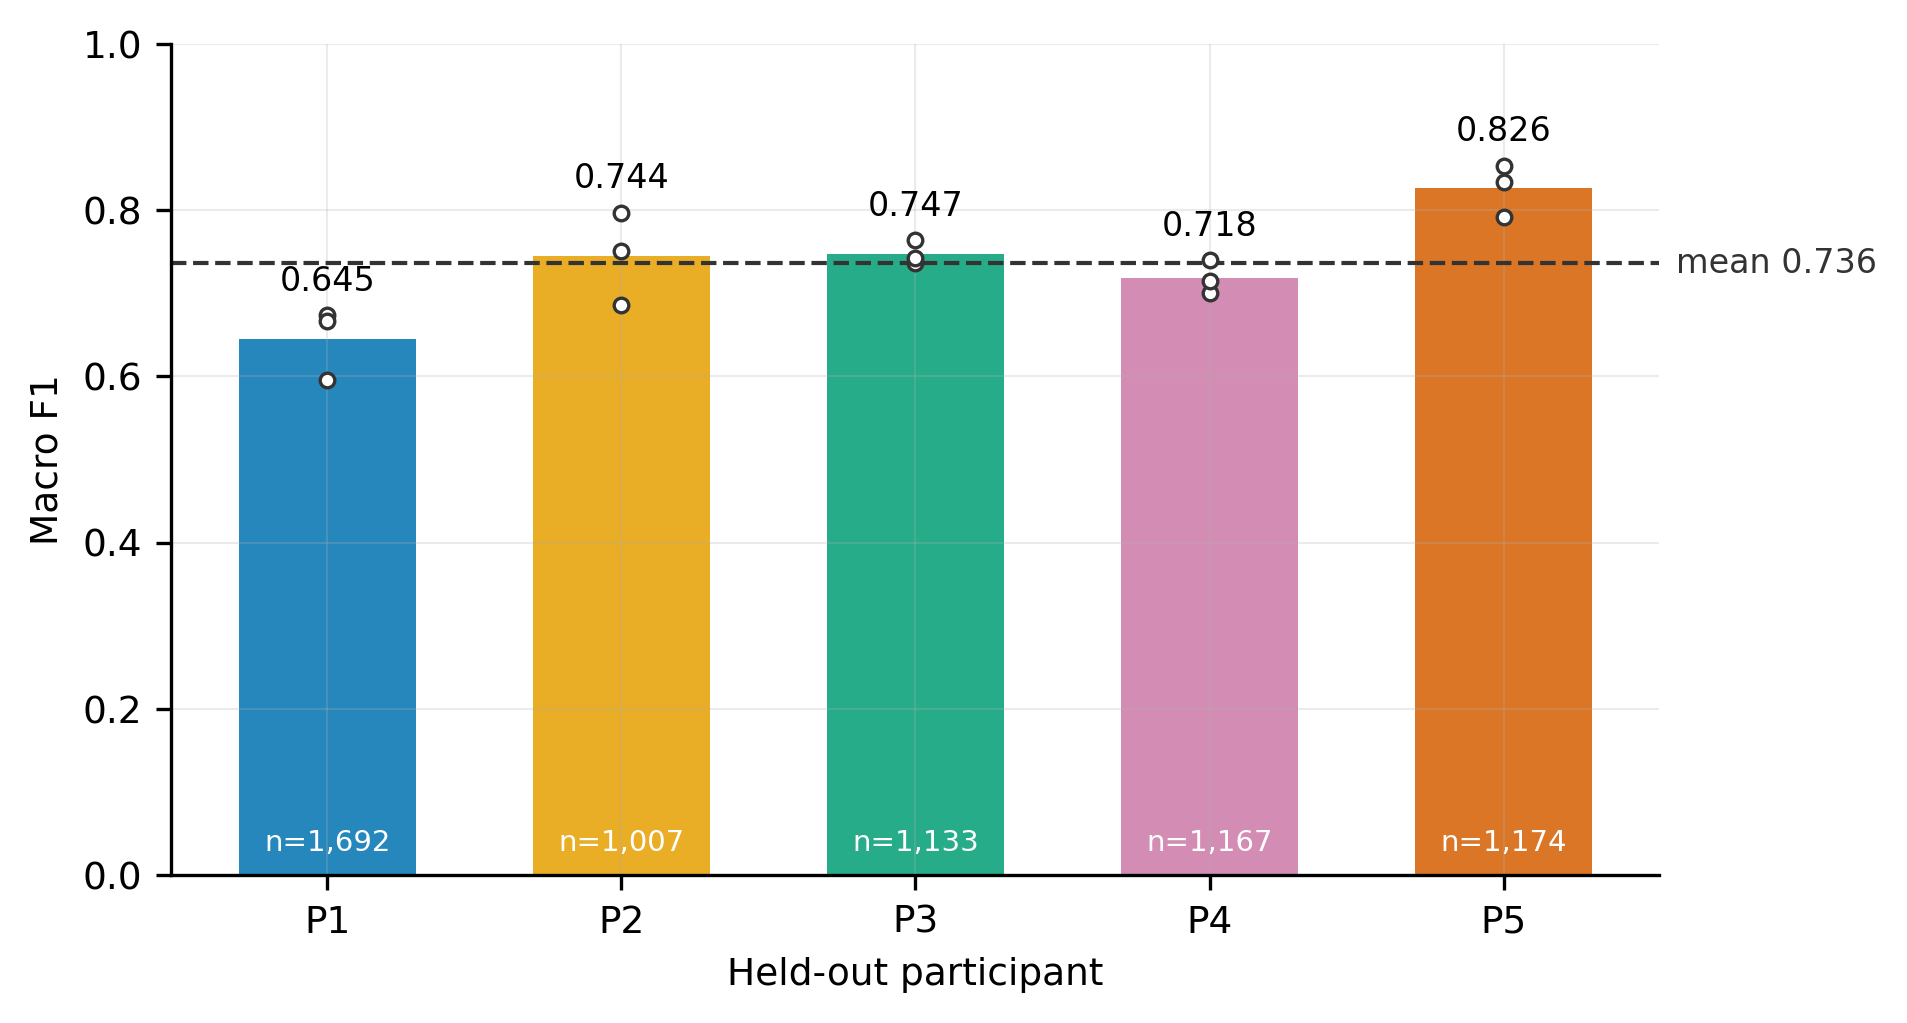
\includegraphics[width=0.72\linewidth]{Figures/five_class_per_participant.png}
  \caption{Macro-F1 for each held-out participant. Each bar is the mean over the three seeds of that participant's own leave-one-subject-out fold, the open markers are the three individual seeds, and the label inside each bar gives that participant's held-out window count. Five participants cannot characterize population variability, so no generalization claim follows from the mean.}
  \Description{Bar chart of per-participant macro F1 with the mean marked.}
  \label{fig:per_participant}
\end{figure*}

\subsection{Training behavior and computational measurements}

Because the final model of each fold is refit for a fixed epoch budget chosen inside that fold, there is no early stopping and no validation set at refit time; the curves in Fig.~\ref{fig:loss_curves} are training-fit diagnostics, and the held-out participant appears in none of them. Budgets ranged from 12 to 43 epochs (median 26) across the fifteen fold--seed combinations, and training loss had largely flattened by the end of each budget. The gap between the final training-fit macro-F1 and the corresponding held-out macro-F1 averaged 0.133 and ranged from 0.022 (participant 5) to 0.269 (participant 1)---the same participant whose windows are the most numerous and the least well ranked. That ordering is the expected signature of between-participant variation rather than of optimization failure.

\begin{figure*}[h]
  \centering
  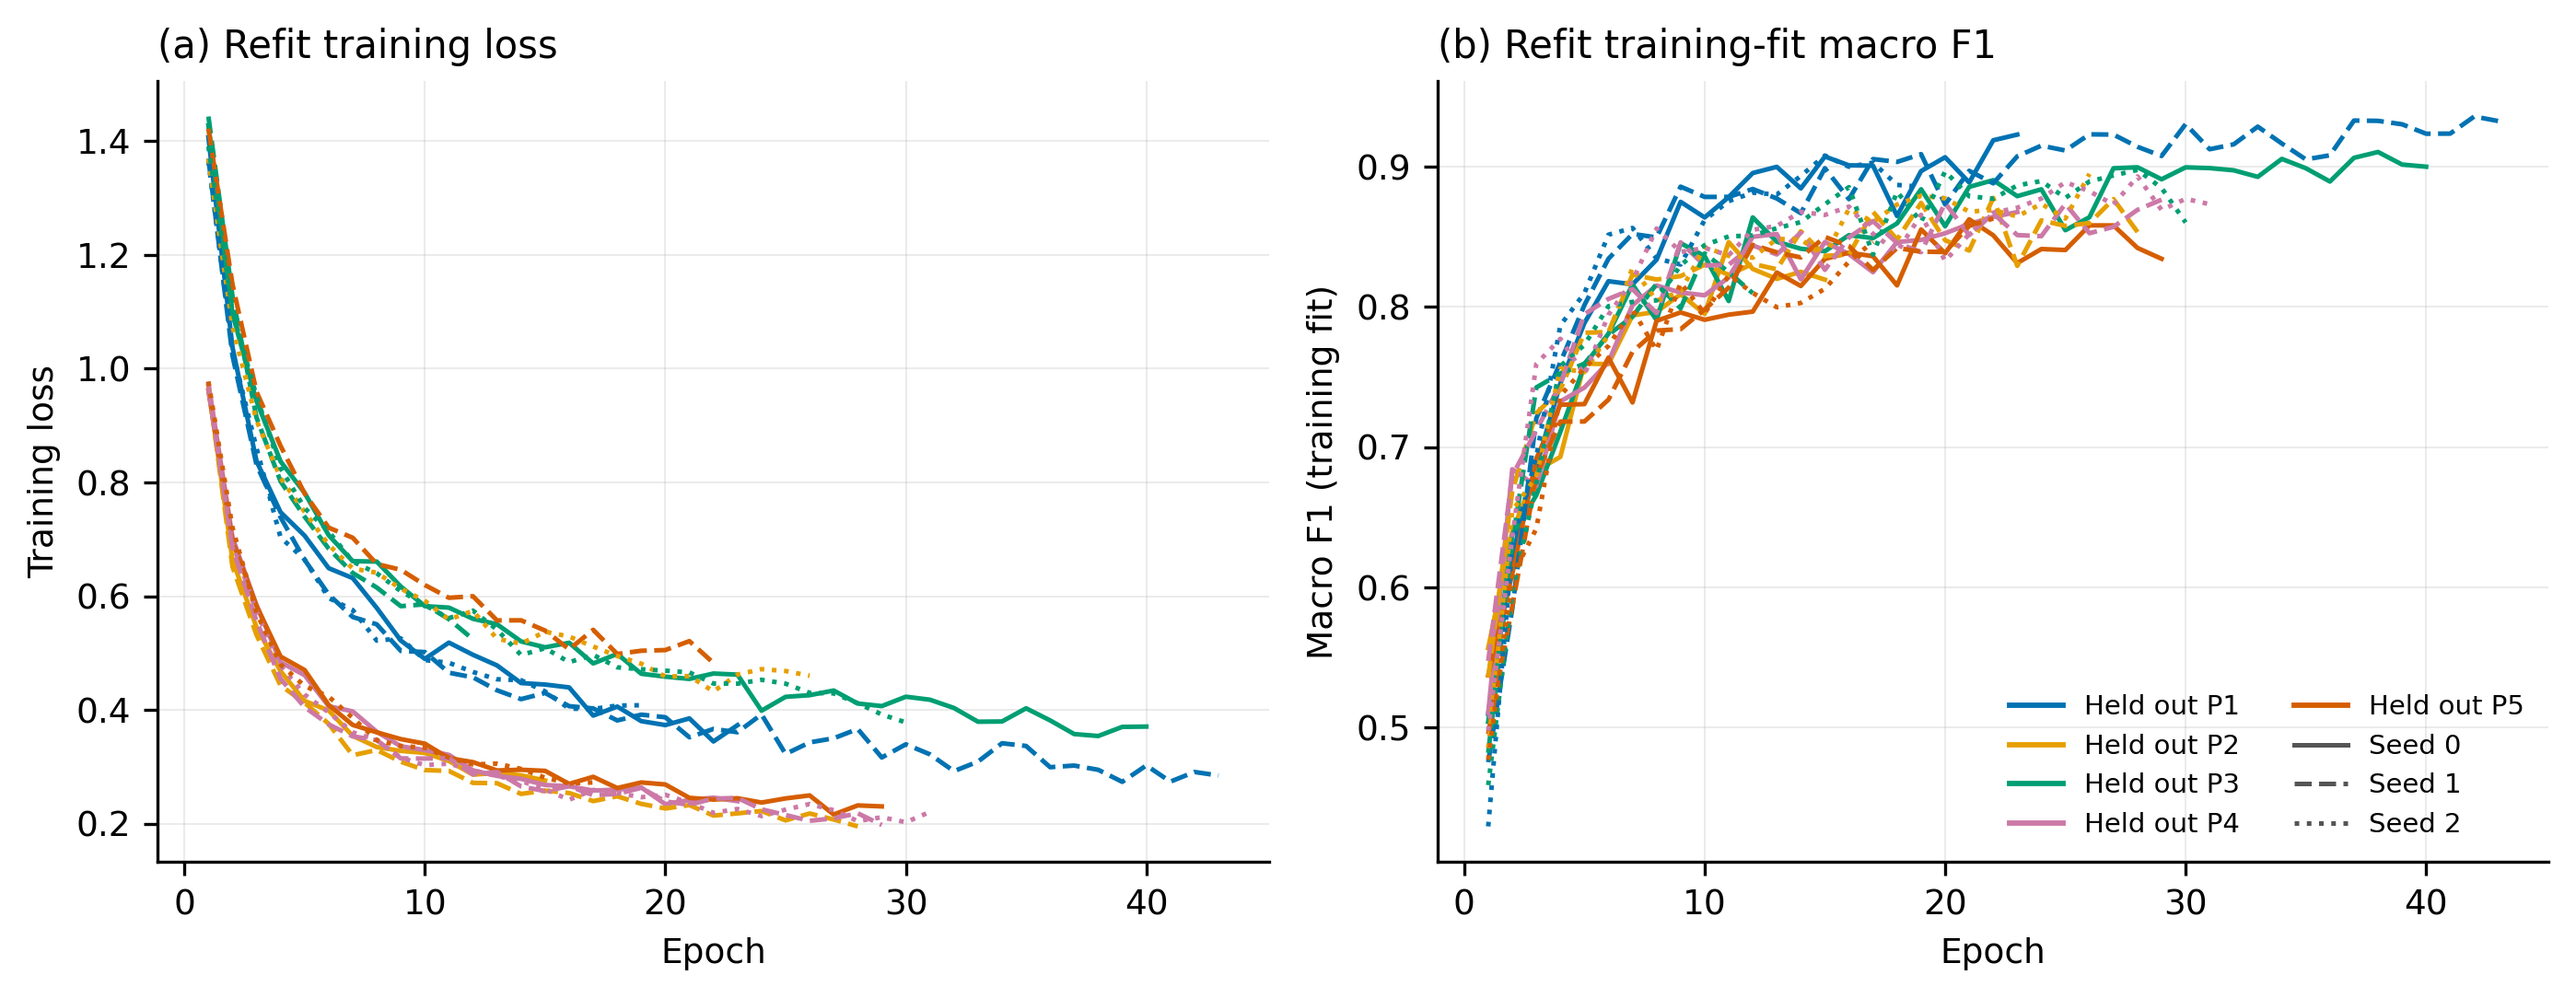
\includegraphics[width=0.92\linewidth]{Figures/training_curves_5class.png}
  \caption{Refit training loss (a) and training-fit macro-F1 (b) for all fifteen fold--seed combinations, colored by held-out participant. Line style encodes the seed: solid seed 0, dashed seed 1, dotted seed 2. Each refit runs for the epoch budget chosen inside its own fold, so the curves end at different epochs. The held-out participant contributes to no curve and is scored once, after training ends.}
  \label{fig:loss_curves}
\end{figure*}

The five-class model contained 7,485 trainable parameters and occupies 29.2~KiB at 32-bit precision. Three latencies must be kept separate. The \emph{input-context latency} is 1000~ms: the window length, and therefore the earliest point at which any decision about an event can exist. The \emph{decision update interval} is 500~ms, the stride. The \emph{processing latency}---filtering, wavelet transform and forward pass for one pre-segmented window on an Intel CPU---is 2.97~ms (2.88~ms forward pass, 95th percentile 2.95~ms, plus 0.08~ms preprocessing), giving an earliest possible decision at 1003~ms. For reference on the same bench, an early-fusion CNN baseline (19,141 parameters) took 0.29~ms and a bidirectional LSTM (10,309 parameters) 1.39~ms.

The compute time alone is not detection latency, and none of these measurements supports a wearable or real-time claim. No streaming implementation exists, the production filter chain is zero-phase and therefore acausal, and the measurements were taken on laptop and desktop hardware. Power consumption, end-to-end latency, wireless synchronization, and reliability on a wearable device remain unmeasured.

\section{Discussion}

\subsection{Engineering interpretation}

Within this dataset, the dual-branch wavelet CNN separated five instructed experimental conditions with a participant-level macro-F1 of 73.6\% and a macro one-vs-rest AUC of 0.962, and it did so under a protocol in which no held-out participant's windows touched normalization, class weighting, augmentation, hyperparameter selection, or training. We do not claim that it outperformed the alternative architectures: that comparison has not been run on the corrected signal, and the only interim evidence---a single-fit screening harness on band energies---puts logistic regression at 0.679 macro-F1 against the network's 0.736 on identical windows and folds, a gap small enough at $N=5$ that it cannot carry an architectural claim in either direction.

Adding quiet rest changed the task from classification among activity windows to discrimination of five experimental conditions including a limited non-event condition, and rest proved to be the most reliably recovered class (92.5\% recall, AUC 0.960). The residual 6.0\% of rest windows assigned to clenching or grinding is the most decision-relevant number in the paper, because it is the closest available analogue of a false alarm.

The audio contribution (RQ2) is not quantified here. The previously reported figure of $+0.035$ macro-F1 was obtained through the defective chain, in which mains harmonics carried the majority of the in-band power, and is withdrawn. Figure~\ref{fig:signal_comparison} illustrates the qualitative contrast that motivates the audio branch. Quiet rest is silent in both modalities. Instructed grinding produces sustained electromyographic activation with comparatively little acoustic energy. Chewing produces rhythmic bursts separated by relaxation intervals, each accompanied by a large acoustic transient roughly five times the amplitude seen during grinding. If that pattern is representative, the audio branch is most likely helping to identify eating rather than to separate clenching from grinding---which is precisely the hypothesis embedded in RQ2 and precisely what the pending ablation, which removes chewing and repeats the modality contrast, is designed to test. We state it here as a hypothesis motivated by the traces, not as a result.

\subsection{What the filter correction changed, and why it is reported}

The single largest determinant of the results in this paper was not the architecture, the loss function, or the fusion strategy. It was whether the mains harmonics were removed. Run over the identical 6,173 windows and folds, the screening harness scored 0.393 macro-F1 (56.0\% accuracy) through the superseded chain and 0.679 (79.7\%) through the corrected one---a step larger than every other change we evaluated combined---and participants whose held-out accuracy had previously sat at or below the five-class chance level moved into the normal range.

The mechanism is easy to state and easy to miss. A chain that notches only the supply fundamental is correct when the fundamental is the dominant interference. Here it was not: the acquisition hardware had already removed it, and what remained was harmonic. A filter-response diagram of that chain looks textbook-correct, and the pipeline was reproducible, version-controlled, and tested; none of that could detect the error, because nothing in the figure set placed the filter response over the measured spectrum of the recordings. When a classifier is trained on such a signal, between-participant differences in interference amplitude can dominate between-condition differences in physiology. In our recordings, correction reduced the between-participant amplitude spread from $5.0\times$ to $3.0\times$ and eliminated all 20 participant pairs in which one person's resting EMG had exceeded another person's active EMG. A model trained before the correction could reduce its loss by learning who a window came from rather than what they were doing, and leave-one-subject-out evaluation is exactly the protocol that then reports the consequence as poor generalization.

We report this at length for three reasons. First, it is the honest provenance of the numbers: the results in this paper are not an incremental improvement on our earlier ones; they replace them, and the two sets are not comparable. Second, the vulnerability is not specific to this dataset. Head-mounted electrodes, long leads, and acquisition software that applies undocumented fixed filtering are common in ambulatory jaw-activity work, and published accuracies are rarely accompanied by a measured interference statistic. Third, the check is cheap: the fraction of in-band power lying within a few hertz of each mains multiple can be computed per recording in seconds, and it separated the contaminated from the clean recordings here by more than an order of magnitude. We suggest that instrumental studies of masticatory-muscle activity report such a statistic alongside their accuracies, and that filter-response figures be drawn over the measured spectrum of the data rather than alone.

\begin{figure*}[h]
  \centering
  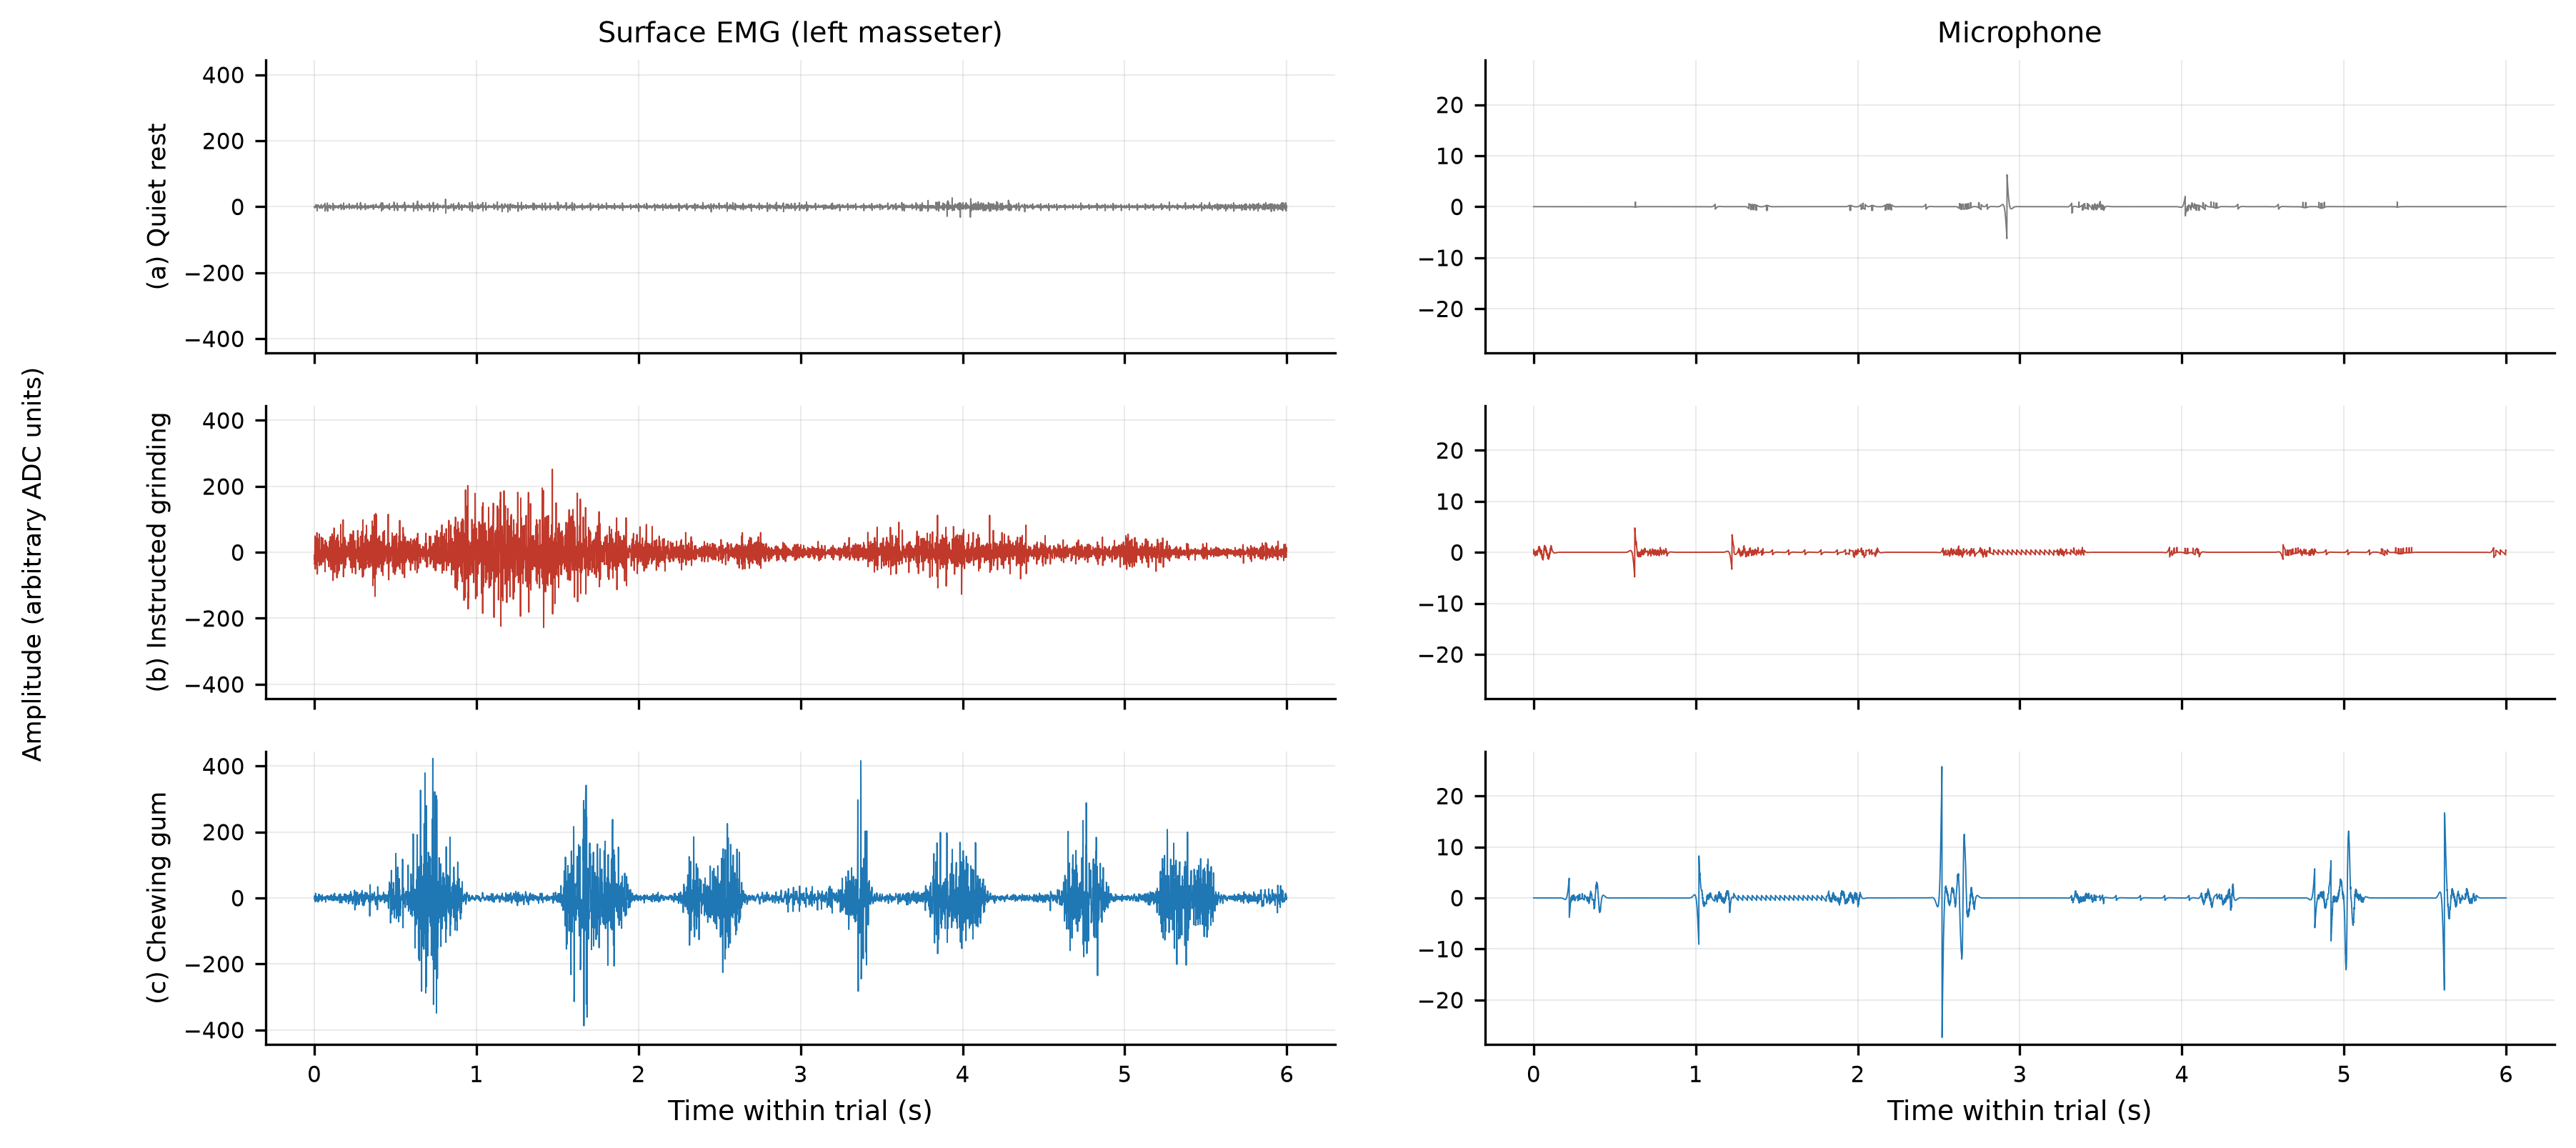
\includegraphics[width=\linewidth]{Figures/signal_comparison_5class.png}
  \caption{Six-second excerpts of one participant's quiet rest, instructed grinding, and gum chewing, after the corrected production filter chain, on a common scale within each column. (a) Rest is quiet in both modalities. (b) Instructed grinding produces sustained EMG activation without a clear burst--relaxation rhythm, and comparatively little acoustic energy. (c) Chewing produces rhythmic EMG bursts separated by relaxation intervals, each accompanied by a large acoustic transient---roughly five times the microphone amplitude seen during grinding. Representative examples are illustrative; they are not a measurement of the modality contribution and not validation against natural bruxism episodes.}
  \Description{Three rows of paired EMG and microphone traces for rest, instructed grinding and chewing.}
  \label{fig:signal_comparison}
\end{figure*}

The current result should be compared cautiously with the greater-than-90\% accuracy reported by Sonmezocak and Kurt using EMG alone~\cite{sonmezocak2021detection}. Their classes included jaw opening, clenching, rhythmic grinding, and fatigue/pain; the present classes include rest, movement, clenching, grinding, and chewing. Dataset composition, preprocessing, sample size, and validation design also differ, and our evaluation is leave-one-subject-out, so every reported number is measured on a participant the model has never seen. A within-participant or window-shuffled split of the same data would score considerably higher without measuring anything about a new user. These studies therefore answer different classification questions, and the numerical accuracies do not show that either method is clinically superior.

The clenching--grinding distinction was retained to test whether the architecture could separate static and lateral tooth-contact tasks. It is the weakest distinction in the model: one fifth of clenching windows were labeled grinding and one seventh of grinding windows were labeled clenching, and the two classes interleave in the learned feature space rather than occupying separate regions. We do not claim that this distinction is always necessary for clinical management. Both are only parts of the wider bruxism construct, and a 1-second window may be genuinely unlabelable when a grinding bout passes through a static clenching phase. The observed confusion therefore reflects both signal overlap and task-label ambiguity, and the collapsed tooth-contact analysis---in which the distinction is not required---is correspondingly stronger (93.6\% accuracy, AUC 0.966).

\subsection{Effect of the chewing class}

Chewing was selected as a relevant functional confound, not as evidence of bruxism. In the five-class model it comprised 58.9\% of the windows and achieved an F1 score of 90.8\%, the highest of any class. Excluding it changed participant-level accuracy from 82.1\% to 79.8\% and macro-F1 from 73.6\% to 77.9\%. The direction of those two changes is the point: a headline accuracy computed over this class distribution is carried substantially by the easiest and largest class, whereas macro-F1 improves once that class is removed because the remaining four are more evenly sized. Reporting both analyses, and reporting macro-F1 alongside accuracy throughout, is what keeps the summary honest.

The post-hoc two-group analysis places quiet rest in the comparison group, which makes it more informative than an activity-only contrast. It must still not be labeled clinical ``bruxism detection.'' Chewing can include tooth contact, clenching may occur without clinically important bruxism, and natural bruxism also includes bracing or thrusting without tooth contact. Quiet laboratory rest is much narrower than unrestricted everyday background behavior. A deployable detector will require continuous-stream onset and offset evaluation, diverse non-event behaviors, false alarms per unit time, and event-level sensitivity and positive predictive value.

\subsection{Clinical interpretation within current bruxism and TMD frameworks}

The present sensors measure muscle and sound patterns, not the biological, psychological, or social meaning of those patterns. Under the biopsychosocial model, the same motor activity may have different context, drivers, and consequences across people and time~\cite{manfredini2026biopsychosocial}. A future device should therefore be positioned as one source of instrumentally based assessment within STAB, combined when appropriate with subject report, clinical examination, psychosocial information, sleep-related factors, medications and substances, and possible consequences~\cite{manfredini2024standardised}.

The manuscript also deliberately avoids claiming that bruxism caused TMD or that classifying a task can diagnose or guide treatment of TMD. INfORM/IADR emphasizes validated history and examination, patient-centered decision-making, and conservative management, and cautions that unsupported technological measurements should not replace standard assessment~\cite{inform2025tmd}. Any future clinical study of this system should predefine its intended use---for example, behavior quantification, biofeedback support, or screening for further assessment---and validate that use against an appropriate reference standard.

The need for precise claims is not semantic alone. Practice surveys show inconsistent assessment and management approaches~\cite{mungia2025approaches}, and studies of students and educational programs identify persistent gaps in bruxism and TMD knowledge~\cite{nasanen2026competence,sangalli2026education}. Labeling an instructed-task classifier as a diagnostic bruxism device could reinforce precisely the conflation that current terminology and education seek to correct.

\subsection{Natural fluctuation and future home measurement}

Laboratory repetitions do not capture the frequency, duration, context, or natural variability of awake behavior. EMA studies demonstrate the value of repeated real-time reports in the natural environment~\cite{bracci2018frequency}; longer observations also show that behavior estimates must be interpreted across days and months rather than from a single session~\cite{colonna2025fluctuation}. Bracci et al.~\cite{bracci2024metrics} recommend selecting subject-based, clinically based, or instrumentally based metrics according to the research question. Colonna et al.~\cite{colonna2023electromyographic} further illustrate the feasibility and challenges of 24-hour home EMG.

A next-stage awake study should combine multi-day audio--EMG with synchronized EMA, a clearly defined background/rest class, and blinded annotation of candidate episodes. Day-level and participant-level performance should be reported, including false positives per hour. Privacy-preserving audio features or on-device feature extraction should be considered before home deployment.

No conclusion about sleep bruxism can be drawn from the present awake laboratory tasks. A sleep study would require overnight data, appropriate sleep staging and event criteria, comparison with a suitable reference such as polysomnography or validated portable assessment, and repeated nights to evaluate night-to-night variability~\cite{cidverdejo2024instrumental}. Separate models may be required for awake and sleep contexts.

\subsection{Validity and limitations}

The principal limitation is the cohort size ($N=5$). The 6,173 overlapping five-class windows provide many optimization examples but do not replace independent participants: adjacent windows share half their samples, and a single participant contributed 27\% of them. Window-level confidence intervals or tests would overstate precision and are deliberately not reported, and LOSO does not establish external generalization when only five people are available. The between-participant spread observed here---accuracy from 72.0\% to 91.7\% and macro-F1 from 64.5\% to 82.6\%---is itself the clearest evidence that a five-person mean is not a population estimate. Age, facial anatomy, subcutaneous tissue, dentition, electrode placement, skin impedance, behavior intensity, and prior diagnosis may all affect EMG and audio signals.

Two results in this manuscript are incomplete rather than negative, and are marked as such. The modality ablation (RQ2) and the architecture comparison (RQ3) have not been run on the corrected signal; both tables carry explicit pending markers, and the screening values quoted for direction come from a harness that fits one model per fold with a feature set chosen after seeing these participants, which makes it optimistic in level. The primary five-class run is complete: all three prespecified seeds finished all five outer folds, and seed-to-seed variation was small (macro-F1 0.717, 0.746 and 0.745) relative to the between-participant spread.

Several analysis choices remain declared but unexercised. Held-out probabilities are uncalibrated (expected calibration error 0.046); temperature scaling is implemented but was not applied, so the scores must not be read as probabilities, though every reported AUC is unaffected. A per-participant normalization scope, which uses the held-out participant's unlabeled signal distribution but never their labels, is implemented and prespecified; a screening estimate values it at roughly $+0.06$ macro-F1, but it is a transductive test-time adaptation that would require a per-user fitting session, and no number in this paper uses it. Similarly, averaging predictions over longer contexts raises screening macro-F1 from 0.735 at one window to 0.821 at about 5.5 seconds; because every recording here contains a single condition, that aggregation approaches a majority vote over a homogeneous trial and is valid only as a labeled trial-level secondary analysis, never as continuous-stream detection. The 1-second window is therefore a constraint of this design rather than a tuned parameter.

Construct validity is limited because the task set covers tooth-contact clenching and grinding but not bracing or thrusting without tooth contact. The participants' prior diagnoses were not independently phenotyped for this study. Criterion validity is not established because no spontaneous episode was verified against a clinical or instrumental reference standard. Ecological validity is limited because participants intentionally performed the tasks in a controlled laboratory. Elicited activities may be more regular, longer, or more forceful than natural activity, making them easier to classify. Device validity is consequently limited to internal discrimination of these instructed task windows.

Including quiet rest removes one limitation of an activity-only design, but the background data remain incomplete. Rest was recorded in a controlled laboratory and did not systematically sample speaking, swallowing, facial expression, head movement, coughing, eating outside the scripted task, environmental noise, or other free-living behaviors. The five-class analysis can estimate confusion against quiet rest---6.0\% of rest windows fell into the clenching/grinding group---but it cannot estimate false alarms per hour during unrestricted use, because the denominator that matters there is unrestricted behavior and this design does not contain any. The current microphone setup also raises privacy and ambient-noise issues that were not tested.

Labels themselves carry residual uncertainty. Class membership rests on a button press confirmed by the experimenter, and the alignment audit showed that muscle activity preceded the marker at four of every five onsets, with a median lag of $-0.075$~s. The 0.25-s transition guard exceeds the median error in the harmful direction and covers the 95th percentile, but 7\% of trial-leading windows may still carry a partially mislabeled edge. The acquisition token for the grinding condition was a filename label chosen at recording time; the corresponding class is reported throughout as instructed grinding, and performing grinding on command is plausibly more regular and easier to detect than spontaneous behavior---a bias in the optimistic direction.

Finally, the modality comparison is algorithm-specific, and here it is also simply unmeasured. A stronger EMG-only architecture, different sensor placement, additional muscles, or calibrated intensity features could all alter whatever fusion benefit the pending ablation reveals. The reported computational measurements were obtained on laptop and desktop hardware rather than a wearable prototype, and the acausal filter chain means they do not describe a streaming system at all.

\section{Conclusion}

This five-participant proof-of-concept study evaluates whether a compact dual-branch wavelet CNN can combine surface EMG and audio to classify quiet rest and four instructed awake jaw activities. Under leakage-free nested leave-one-subject-out evaluation on corrected signals, the fused model achieved a participant-level accuracy of 82.1\%, a macro-F1 of 73.6\%, and a macro one-vs-rest AUC of 0.962, with per-participant accuracy ranging from 72.0\% to 91.7\%. Excluding chewing yielded 79.8\% accuracy and 77.9\% macro-F1 across rest, movement, clenching, and grinding. The collapsed clenching/grinding-versus-rest/movement/chewing analysis achieved an F1 of 87.3\% and an AUC of 0.966, with 6.0\% of quiet-rest windows falling on the tooth-contact side. The modality ablation and the baseline architecture comparison are prespecified but not yet run, and are reported as pending rather than estimated from the superseded pipeline.

A second conclusion is methodological. The dominant factor in these results was not the model but the measurement chain: correcting a filter that removed an absent mains fundamental while passing the harmonics that carried 91.3--99.8\% of the in-band power changed the pipeline's screening macro-F1 by more than every other intervention we evaluated combined, and eliminated cases in which one participant's resting EMG exceeded another's active EMG. We recommend that instrumental studies of masticatory-muscle activity report a measured interference statistic beside their accuracies and plot filter responses over the measured spectrum of their own recordings.

The study does not validate a bruxism diagnostic device. Although quiet-rest windows are now included, the study did not include bracing or thrusting, unrestricted background behavior, spontaneous awake episodes, sleep recordings, or an independent clinical reference standard. The defensible conclusion is therefore technical: modality-specific audio--EMG fusion merits further evaluation for distinguishing instructed jaw activities from quiet rest in a larger, phenotyped, multi-day continuous-recording study designed around current bruxism terminology and clinical assessment frameworks.

\backmatter

\section*{Data availability}
The datasets generated and/or analyzed during the current study are not publicly available because of participant-privacy restrictions but are available from the corresponding author on reasonable request, subject to institutional and ethical requirements.

\section*{Code availability}
The custom code used for signal preprocessing, wavelet decomposition, model training, and evaluation is available from the corresponding author on reasonable request. Every number and figure in this manuscript was regenerated from a saved prediction ledger in which each held-out window appears exactly once per task, model, modality and seed, together with its full probability vector, the source commit, and hashes of the resolved configuration, the data manifest, the window index and the model checkpoint. The run reported here is \texttt{five\_class\_nested\_loso\_}\allowbreak\texttt{20260807T211827\_2b6fb5ac}, carrying configuration hash \texttt{2b6fb5ac}, manifest hash \texttt{7ebbcc8d} and window-index hash \texttt{b2cf690c}.

\section*{Funding declaration}
Research reported in this publication was supported by an award from the Rhode Island Life Science Hub Small Grant Program (Principal Investigator T. A. Walls; Co-Investigators R. Abiri and M. Furmanek). The project was also partially supported by National Science Foundation grant 2245558 (Principal Investigator R. Abiri).

\section*{Acknowledgements}
We thank University of Rhode Island undergraduate and graduate students Anjolaoluwa Akingbile, Jessica Constantine, and Nathan DeSalvo, who located and summarized the functions of bruxism devices before this project.

\section*{Author contributions}
M.H.F.: methodology, software, analysis, writing---original draft, and writing---review and editing. A.R.: protocol development, software, data curation, data collection, formal analysis, and review and editing. R.S.: methodology, validation, and writing---review and editing. M.P.F.: conceptualization and study design, research-grant development, protocol development, and manuscript revision. R.A.: conceptualization, project administration, resources, supervision, and writing---review and editing. T.A.W.: conceptualization, research-grant authorship, protocol development, project oversight, and manuscript revision. All authors reviewed and approved the final manuscript.

\section*{Competing interests}
The authors declare no competing interests.

\begin{thebibliography}{99}

\bibitem{lobbezoo2018international}
Lobbezoo, F. \emph{et al.} International consensus on the assessment of bruxism: report of a work in progress. \emph{J. Oral Rehabil.} \textbf{45}, 837--844 (2018).

\bibitem{manfredini2024standardised}
Manfredini, D. \emph{et al.} Standardised Tool for the Assessment of Bruxism. \emph{J. Oral Rehabil.} \textbf{51}, 29--58 (2024).

\bibitem{colonna2023electromyographic}
Colonna, A., Noveri, L., Ferrari, M., Bracci, A. \& Manfredini, D. Electromyographic assessment of masseter muscle activity: a proposal for a 24 h recording device with preliminary data. \emph{J. Clin. Med.} \textbf{12}, 247 (2023).

\bibitem{gul2024advanced}
Gul, J. Z., Yang, B.-S., Kuo, Y.-C., Hsu, W.-H. \& Su, F.-C. Advanced sensing system for sleep bruxism across multiple postures via EMG and machine learning. \emph{Sensors} \textbf{24}, 5426 (2024).

\bibitem{stuginski2016detection}
Stuginski-Barbosa, J., Porporatti, A. L., Costa, Y. M., Svensson, P. \& Conti, P. C. R. Agreement of the International Classification of Sleep Disorders criteria with polysomnography for sleep bruxism diagnosis. \emph{J. Prosthet. Dent.} \textbf{117}, 61--66 (2017).

\bibitem{raez2006techniques}
Raez, M. B. I., Hussain, M. S. \& Mohd-Yasin, F. Techniques of EMG signal analysis: detection, processing, classification and applications. \emph{Biol. Proced. Online} \textbf{8}, 11--35 (2006).

\bibitem{castroflorio2013use}
Castroflorio, T., Mesin, L., Tartaglia, G. M., Sforza, C. \& Farina, D. Use of electromyographic and electrocardiographic signals to detect sleep bruxism episodes in a natural environment. \emph{IEEE J. Biomed. Health Inform.} \textbf{17}, 994--1001 (2013).

\bibitem{sonmezocak2021detection}
Sonmezocak, T. \& Kurt, S. Detection of EMG signals by neural networks using autoregression and wavelet entropy for bruxism diagnosis. \emph{Elektron. Elektrotechn.} \textbf{27}, 11--21 (2021).

\bibitem{heyat2020computational}
Heyat, M. B. B. \emph{et al.} Computational ensemble expert system classification for the recognition of bruxism using physiological signals. \emph{Appl. Sci.} \textbf{10}, 7410 (2020).

\bibitem{lan2022comparative}
Lan, K.-W., Jiang, L.-L. \& Yan, Y. Comparative study of surface electromyography of masticatory muscles in patients with different types of bruxism. \emph{World J. Clin. Cases} \textbf{10}, 6876--6889 (2022).

\bibitem{romano2024wearable}
Romano, F. \emph{et al.} Toward wearables for bruxism detection: voluntary oral behaviors sound recorded across the head depend on transducer placement. \emph{Clin. Exp. Dent. Res.} \textbf{10}, e70001 (2024).

\bibitem{martinot2021artificial}
Martinot, J.-B. \emph{et al.} Artificial intelligence analysis of mandibular movements enables accurate detection of phasic sleep bruxism in OSA patients: a pilot study. \emph{Nat. Sci. Sleep} \textbf{13}, 1449--1459 (2021).

\bibitem{haugland2020automatic}
Haugland, M., Christiansen, C. \& Takano, N. Automatic detection of teeth clenching and/or teeth grinding. US Patent 10,736,560 (2020).

\bibitem{patwa2017bruxism}
Patwa, A. N. \& Patwa, M. N. Bruxism detection system with chin-mounted accelerometer sensor. US Patent Application 2017/0265801 (2017).

\bibitem{englehart2003robust}
Englehart, K. \& Hudgins, B. A robust, real-time control scheme for multifunction myoelectric control. \emph{IEEE Trans. Biomed. Eng.} \textbf{50}, 848--854 (2003).

\bibitem{phinyomark2012feature}
Phinyomark, A., Phukpattaranont, P. \& Limsakul, C. Feature reduction and selection for EMG signal classification. \emph{Expert Syst. Appl.} \textbf{39}, 7420--7431 (2012).

\bibitem{chowdhury2013surface}
Chowdhury, R. H. \emph{et al.} Surface electromyography signal processing and classification techniques. \emph{Sensors} \textbf{13}, 12431--12466 (2013).

\bibitem{faust2018deep}
Faust, O., Hagiwara, Y., Hong, T. J., Lih, O. S. \& Acharya, U. R. Deep learning for healthcare applications based on physiological signals: a review. \emph{Comput. Methods Programs Biomed.} \textbf{161}, 1--13 (2018).

\bibitem{tsinganos2019improved}
Tsinganos, P., Cornelis, B., Cornelis, J., Jansen, B. \& Weiss, A. Improved gesture recognition based on sEMG signals and temporal convolutional networks. \emph{IEEE Access} \textbf{7}, 154853--154863 (2019).

\bibitem{lin2017focal}
Lin, T.-Y., Goyal, P., Girshick, R., He, K. \& Doll\'ar, P. Focal loss for dense object detection. In \emph{Proc. IEEE Int. Conf. Computer Vision}, 2980--2988 (2017).

\bibitem{johnson2019survey}
Johnson, J. M. \& Khoshgoftaar, T. M. Survey on deep learning with class imbalance. \emph{J. Big Data} \textbf{6}, 27 (2019).

\bibitem{vandermaaten2008visualizing}
van der Maaten, L. \& Hinton, G. Visualizing data using t-SNE. \emph{J. Mach. Learn. Res.} \textbf{9}, 2579--2605 (2008).

\bibitem{bharathi2025unveiling}
Bharathi, B. M. R., Balaji, N. S., Meena, R. \& Sekar, M. R. C. Unveiling optimal mother wavelets by COPRAS method: analyzing speech signals despite face mask and shield obstacles. \emph{Sci. Rep.} \textbf{15}, 14044 (2025).

\bibitem{verhoeff2025definitions}
Verhoeff, M. C. \emph{et al.} Updating the bruxism definitions: report of an international consensus meeting. \emph{J. Oral Rehabil.} \textbf{52}, 1335--1342 (2025). doi:10.1111/joor.13985.

\bibitem{manfredini2026biopsychosocial}
Manfredini, D. \& Lobbezoo, F. The biopsychosocial model of bruxism. \emph{Cranio}, 1--9 (2026). doi:10.1080/08869634.2026.2655187.

\bibitem{manfredini2024evolution}
Manfredini, D. The evolution of a field: a challenge and an opportunity. \emph{Cranio} \textbf{42}, 251--252 (2024). doi:10.1080/08869634.2024.2320624.

\bibitem{inform2025tmd}
Manfredini, D. \emph{et al.} Temporomandibular disorders: INfORM/IADR key points for good clinical practice based on standard of care. \emph{Cranio} \textbf{43}, 1--5 (2025). doi:10.1080/08869634.2024.2405298.

\bibitem{mungia2025approaches}
Mungia, R. \emph{et al.} Dental practitioner approaches to bruxism: preliminary findings from the National Dental Practice-Based Research Network. \emph{Cranio} \textbf{43}, 480--488 (2025). doi:10.1080/08869634.2023.2192173.

\bibitem{nasanen2026competence}
N\"as\"anen, J. \emph{et al.} Self-assessed competence in relation to bruxism among undergraduate dental students in Finland. \emph{Cranio} \textbf{44}, 160--170 (2026; published online 2025). doi:10.1080/08869634.2025.2472085.

\bibitem{sangalli2026education}
Sangalli, L. Evolving progress in temporomandibular disorder education for predoctoral dental programs. \emph{Cranio} \textbf{44}, 181--183 (2026; published online 2025). doi:10.1080/08869634.2025.2543482.

\bibitem{bracci2024metrics}
Bracci, A. \emph{et al.} Research routes on awake bruxism metrics: implications of the updated bruxism definition and evaluation strategies. \emph{J. Oral Rehabil.} \textbf{51}, 150--161 (2024). doi:10.1111/joor.13514.

\bibitem{bracci2018frequency}
Bracci, A., Djukic, G., Favero, L., Salmaso, L., Guarda-Nardini, L. \& Manfredini, D. Frequency of awake bruxism behaviors in the natural environment: a seven-day, multiple-point observation of real-time report in healthy young adults. \emph{J. Oral Rehabil.} \textbf{45}, 423--429 (2018). doi:10.1111/joor.12627.

\bibitem{colonna2025fluctuation}
Colonna, A., Lobbezoo, F., Bracci, A., Ferrari, M., Val, M. \& Manfredini, D. Long-term study on the fluctuation of self-reported awake bruxism in a cohort of healthy young adults. \emph{J. Oral Rehabil.} \textbf{52}, 37--42 (2025). doi:10.1111/joor.13872.

\bibitem{cidverdejo2024instrumental}
Cid-Verdejo, R. \emph{et al.} Instrumental assessment of sleep bruxism: a systematic review and meta-analysis. \emph{Sleep Med. Rev.} \textbf{74}, 101906 (2024). doi:10.1016/j.smrv.2024.101906.

\end{thebibliography}

\end{document}
